% usobasico.tex
%
% Copyright (C) 2022--2026 José A. Navarro Ramón <janr.devel@gmail.com>
% Licencia del código GPLv2
% Licencia Creative Commons Recognition Non-Commercial Share-alike.
% (CC-BY-NC-SA)


\chapter{Uso Básico}
Este capítulo tiene los siguientes objetivos:
\begin{enumerate}
\item Aprender cómo cargar el paquete en Lua\LaTeX.
\item Familiarizarse con sus principales características, sobre todo las que se aplican
  en un contexto de ESO y bachillerato.
\item Conocer algunas formas de personalizar las fórmulas y/o reacciones químicas con
  respecto a las que presenta por defecto el paquete.
\item Conocer sus puntos fuertes y carencias.
\end{enumerate}

\section{Introducción}
En esta sección veremos algunos detalles importantes para usar este paquete.

\subsection{¿Cuándo interesa utilizarlo?}
Este paquete de química es más complejo que \textsf{mhchem}
Sirve para escribir:
\begin{enumerate}
\item Compuestos orgánicos (o inorgánicos, sobre todo cuando se muestran los enlaces).
\item Reacciones químicas complejas donde aparecen compuestos orgánicos e inorgánicos.
\end{enumerate}

Se recomienda utilizar \textsf{mhchem} en las situaciones que se mostraron en el
capítulo anterior. Por tanto, es recomendable repasar el paquete del capítulo anterior.
En algunos de esos casos también se podría utilizar también \textsf{chemfig}, aunque
teniendo que escribir más. En algunas de esas situaciones especiales podría interesar
\textsf{chemfig}, personalizando algo la fórmula.

En realidad, \textsf{chemfig} tiene muchas formas de personalizar las fórmulas y/o
reacciones químicas, mientras que \textsf{mhchem} es más limitado en ese sentido.

\subsection{Carga de \textsf{chemfig}}
Para poder utilizarlo es preciso cargarlo en el preámbulo del documento, esto es,
antes de \texttt{\textbackslash begin
  \{document\}...\textbackslash end\{document\}}.

Se pueden dar dos situaciones:
\vspace{-1ex}
\begin{itemize}
\item Si \textsf{chemfig} se carga en el fichero principal:
  \ttres{\textbackslash usepackage\{chemfig\}}
\item Si queremos que el fichero principal se vea más ordenado, entonces se debe
  indicar qué otro fichero realizará la carga, en cuyo caso se deberá escribir en
  el principal la línea: 
  \ttres{\textbackslash usepackage\{fichero.pkg\}} en el
  principal, indicando que el fichero que realizará la carga será 
 \texttt{fichero.pkg.sty}. En este último hay que añadir una línea que ponga:
 \ttres{\textbackslash RequirePackage\{chemfig\}},
 además del resto de paquetes que nos interese cargar.
\end{itemize}

\vspace{3ex}

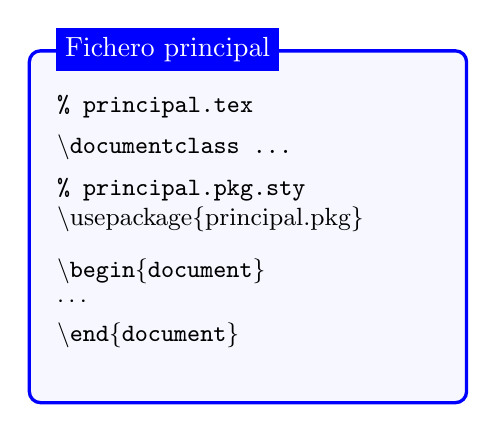
\begin{tikzpicture}
  % Define box and box title style
  \tikzstyle{myboxfichero} = [draw=blue, fill=blue!3, very thick,
  rectangle, rounded corners, inner sep=10pt, inner ysep=20pt]
  \tikzstyle{fancytitle} =[fill=blue, text=white]
    
  \node [myboxfichero] (box){%
    \begin{minipage}{0.40\textwidth}
      {\small
        
        \vspace{-1ex}
        \texttt{\% principal.tex}
        
        \vspace{1ex}
        
        \texttt{\textbackslash documentclass ...}
        
        \vspace{1ex}
        
        \texttt{\% principal.pkg.sty}
        
        \ttres{\textbackslash usepackage\{principal.pkg\}}
        
        \vspace{2ex}
        
        \texttt{\textbackslash begin\{document\}}
        
        \texttt{$\cdots$}
        
        \texttt{\textbackslash end\{document\}}
      }
    \end{minipage}
  };

  \node[fancytitle, right=10pt] at (box.north west) {Fichero principal};
  % \node[fancytitle, rounded corners] at (box.east) {$\clubsuit$};
\end{tikzpicture}%
%
\hspace{1em}
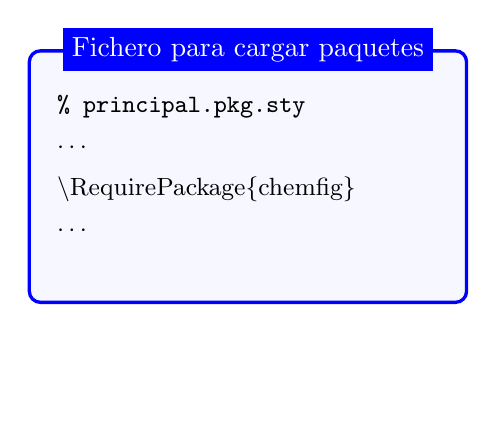
\begin{tikzpicture}[transform shape, rotate=0, baseline=-2.9cm]
  % Define box and box title style
  \tikzstyle{myboxfichero} = [draw=blue, fill=blue!3, very thick,
  rectangle, rounded corners, inner sep=10pt, inner ysep=20pt]
  \tikzstyle{fancytitle} =[fill=blue, text=white]
  
  \node [myboxfichero] (box) {%
    \begin{minipage}[t!]{0.40\textwidth}
      {\small
        \vspace{-1ex}
        \texttt{\% principal.pkg.sty}
        
        \vspace{1ex}
        
        \texttt{$\cdots$}
        \vspace{1ex}
        
        \ttres{\textbackslash RequirePackage\{chemfig\}}
        \vspace{1ex}
        
        \texttt{$\cdots$}
        
        \vspace{1ex}
      }
    \end{minipage}
  };
  \node[fancytitle] at (box.north) {Fichero para cargar paquetes};
\end{tikzpicture}


\subsection{Uso de \textsf{chemfig}}
El comando básico es \texttt{\textbackslash chemfig\{...\}}.
Su uso genérico es:
\begin{center}
\texttt{\textbackslash chemfig[lista de <claves>=<valores>]\{<código de la molécula>\}}
\end{center}

Antes de seguir mostramos una tabla con las diferentes claves, sus valores por defecto y
significado:
{\small
\begin{center}
  \begin{longtable}{rcl}\hline
    \label{tbl:chemfig_claves}
    \texttt{<clave>} & \texttt{Valor} & \texttt{Descripción}\\\hline
    \texttt{\color{Blue}{chemfig style}}
    & ---
    & Estilo que se le pasa a \textsf{TikZ}\\
    \texttt{\color{Blue}{use atom strut}}
    & \texttt{false}
    & Tener en cuenta la caja de un átomo al situar\\&& la del siguiente\\
    \texttt{\color{Blue}{atom style}}
    & ---
    & Estilo de los nodos \textsf{TikZ} de los átomos\\
    \texttt{\color{Blue}{bond join}}
    & \texttt{false}
    & Une enlaces de forma precisa\\
    \texttt{\color{Blue}{fixed length}}
    & \texttt{false}
    & Todos los enlaces tienen la misma longitud\\
    \texttt{\color{Blue}{cram rectangle}}
    & \texttt{false}
    & No respeta el enlace triangular entre átomos\\
    \texttt{\color{Blue}{cram width}}
    & \texttt{1.5ex}
    & Anchura de la base del enlace \emph{cram}\\
    \texttt{\color{Blue}{cram dash width}}
    & \texttt{1pt}
    & Grosor de cada guión que forma el enlace \emph{cram}\\
    \texttt{\color{Blue}{cram dash sep}}
    & \texttt{2pt}
    & Espacio entre guiones del enlace \emph{cram}\\
    \texttt{\color{Blue}{atom sep}}
    & \texttt{3em}
    & Separación entre átomos\\
    \texttt{\color{Blue}{bond offset}}
    & \texttt{2pt}
    & Espacio entre átomo y enlace\\
    \texttt{\color{Blue}{double bond sep}}
    & \texttt{2pt}
    & Espacio entre líneas en enlaces múltiples\\
    \texttt{\color{Blue}{angle increment}}
    & \texttt{45}
    & Incremento de ángulo cuando se usa código\\
    \texttt{\color{Blue}{node style}}
    & ---
    & Estilo de átomos\\
    \texttt{\color{Blue}{bond style}}
    & ---
    & Estilo de enlaces\\
    \texttt{\color{Blue}{baseline}}
    & \texttt{0pt}
    & Se elige el átomo que define la altura base\\
    \texttt{\color{Blue}{debug}}
    & \texttt{false}
    & Muestra líneas y cajas en la fórmula\\
    \texttt{\color{Blue}{cycle radius coeff}}
    & \texttt{0.75}
    & Controla tamaño del círculo aromático\\
    \texttt{\color{Blue}{stack sep}}
    & \texttt{1.5pt}
    & Espaciado vertical entre argumentos de las\\&& macros \texttt{\textbackslash chemabove} y \texttt{\textbackslash chembelow}\\
    \texttt{\color{Blue}{show cntcycle}}
    & \texttt{false}
    & Muestra numeración en los ciclos\\
    \texttt{\color{Blue}{autoreset cntcycle}}
    & \texttt{true}
    & Reinicia numeración en \texttt{\textbackslash chemfigexecution}\\
    \texttt{\color{Blue}{gchemname}}
    & \texttt{true}
    & Utiliza las asignaciones de profundidad en \\&& \texttt{\textbackslash chemnameinit} y \texttt{\textbackslash chemnameglobal}\\
    \hline
    \caption{Tabla de claves del comando \texttt{\backslash config}.}
  \end{longtable}
\end{center}
}

\vspace{-5ex}
Estas claves se muestran aquí como referencia. Las más importantes se discutirán en las
siguientes secciones.

A veces queremos modificar una opción por defecto para todo el documento, y otras
solo queremos que afecte a una fórmula o grupo de ellas:
\begin{itemize}
\item Para modificar el valor de una clave para todo el documento, podemos
  escribir en el prólogo del documento:
  \begin{center}
    \texttt{\textbackslash setchemfig\{clave=valor\}}
  \end{center}
  \item Para modificar el valor y que afecte a una fórmula, escribiríamos:
    \begin{center}
      \texttt{\textbackslash chemfig[clave=valor]\{... fórmula ...\}}
    \end{center}
\end{itemize}

Puede ser que alguna de las opciones que \textsf{chemfig} nos ofrece por defecto, por
ejemplo, la separación entre los átomos y longitud de los enlaces que nos parecieran
desproporcionadas (véase la tercera celda de la tabla de ejemplos de la sección
siguiente). En ese caso, deberíamos poder modificar esas opciones.

En ese supuesto, sería práctico poner otros valores por defecto que nos parecieran
razonables en el prólogo para todo el documento, y si quisiéramos personalizar alguna fórmula en particular dentro de este, podríamos asignar un valor concreto en ese caso,
sin afectar al resto de fórmulas.


\section{Fórmulas sencillas}
Para las fórmulas (y las reacciones químicas) sencillas se recomienda el paquete
\textsf{mhchem}, que es más fácil de utilizar.
Como primer ejemplo, veamos la fórmula molecular genérica de un alcano:

\vspace{1ex}
\begin{tabular}{|c|}\hline
  \vphantom{$\dfrac{1}{1}$} 
  \chemfig{C_nH_{2n+2}}\\
  \texttt{\textbackslash chemfig\{C\_nH\_(2n+2)\}}\\\hline
\end{tabular}

\vspace{1ex}
 Otras fórmulas:

\begin{tabular}{|c|c|c|c|}\hline
  \vphantom{$\dfrac{1}{1}$} 
  \chemfig{NH_3}
  & \ce{H2}
  & \chemfig{CH_2=CH_2}
  & \ce{CH2=CH2}\\
  \texttt{\textbackslash chemfig\{NH\_3\}}
  & \texttt{\textbackslash ce\{H2\}}                
  & \texttt{\textbackslash chemfig\{CH\_2=CH\_2\}}
  &\texttt{\textbackslash ce\{CH2=CH2\}}\\\hline
\end{tabular}

\vspace{2ex}
 ¿Se podría arreglar la fórmula del eteno en \textsf{chemfig}? Sí:

\vspace{1ex}
\begin{tabular}{|c|c|}\hline
  \vphantom{$\dfrac{1}{1}$} 
  \chemfig[atom sep=1.8em]{CH_2=CH_2}
  & \ce{CH2=CH2}\\
  \texttt{\textbackslash chemfig\ttres{[atom sep=1.8em]}\{CH\_2=CH\_2\}}
  &\texttt{\textbackslash ce\{CH2=CH2\}}\\\hline
\end{tabular}

Más adelante se propondrán unos valores por defecto para \textsf{chemfig}, si se
considera que los que vienen con el paquete no nos interesan.

\vspace{1ex}
 Como se puede observar, cuesta más trabajo, aunque se puede ajustar mejor la
distancia entre los átomos y por tanto, la longitud del enlace;
en este ejemplo vemos un parámetro de la tabla \ref{tbl:chemfig_claves}, que especifica
la distancia entre los \emph{átomos} que forman un enlace. Este valor es global para
la fórmula, pero no afecta a otras fórmulas:
\begin{center}
  \texttt{atom sep=1.8em}
\end{center}
que se reducimos a casi la mitad de su valor por defecto \texttt{3em} y, como
consecuencia, el enlace doble disminuye de tamaño.

La solución, que veremos después, es modificar los valores por defecto para las
distancias interatómicas y otros parámetros en el preámbulo del documento, con lo
que no estaremos obligados a detallarlos en cada fórmula. De esa manera, solo tendremos
que retocar algunos de ellos en fórmulas concretas cuando interese.

\subsection{Estado de agregación}
Se puede añadir el estado de agregación fuera del comando porque \textsf{chemfig} solo
considera los elementos que forman la sustancia, y el estado de agregación no da esa
información (aunque sí de cómo están agregados):

\begin{tabular}{|c|c|c|}\hline
  \vphantom{$\dfrac{1}{1}$}
  \chemfig{Ca}(s)
  & \ce{H2O(l)}
  & \ce{He(g)}\\
  \texttt{\textbackslash chemfig\{Ca\}}\ttres{(s)}
  & \texttt{\textbackslash ce\{H2O\}(l)}
  & \texttt{\textbackslash ce\{He(g)\}}\\\hline
\end{tabular}

\subsection{Sales con paréntesis}
En \textsf{chemfig} es necesario encerrar los paréntesis entre llaves, pues por defecto,
\textsf{chemfig} considera los paréntesis como una ramificación, como veremos más
adelante.

\begin{tabular}{|c|c|}\hline
  \vphantom{\rule{0.4pt}{3ex}}
  \chemfig{Ca{(NO_3)}_2}
  & \chemfig{{(NH4)}_2SO_3}\\
  \texttt{\textbackslash chemfig\{Ca\ttres{\{(NO\_3)\}}\_2\}}
  & \texttt{\textbackslash chemfig\{\ttres{\{(NH\_4)\}}\_2SO\_3\}}\\\hline
\end{tabular}

\subsection{Iones}
Como usuario de \LaTeX, ya sabes que lo primero que hay que tener en cuenta en
\textsf{chemfig} es que las cargas de los iones se especifican como superíndices y
deben escribirse después del acento circunflejo "\texttt{\textasciicircum}".
Pero en \textsf{chemfig} hay que tener en cuenta más detalles.

En la fórmula de la izquierda, el guión (o signo negativo) es interpretado por
\textsf{chemfig} como un enlace sencillo que no puede aparecer como superíndice, por lo
que se produce un error de compilación\footnotemark{}.
Este error se indica, marcando en rojo sin resaltar, el código correspondiente.
\footnotetext{Este problema no se presenta, sin embargo, con el signo "\texttt{+}" de una
  carga positiva.}

En la fórmula del centro esto se evita encerrando el guión entre llaves.
Pero ahora surge otro problema, el resultado no sigue las indicaciones de la IUPAC porque
se recomienda que la carga esté a la derecha de un subíndice. Este error se indica
también en rojo sin resaltar.

A la derecha, se escribe la fórmula correcta encerrando el grupo de átomos entre llaves.
La solución correcta se señala en color rojo resaltado:

 \begin{tabular}{|c|c|c|}\hline
 \vphantom{\rule{0.4pt}{3ex}}
  \texttt{Error} & \chemfig{NO_2^{-}} & \chemfig{{NO_2}^{-}}\\
  \ttbad{\textbackslash chemfig\{NO\_2\textasciicircum -\}}
  & \ttbad{\textbackslash chemfig\{NO\_2\textasciicircum \{-\}\}}
  & \texttt{\textbackslash chemfig\{\ttres{\{NO\_2\}\textasciicircum \{-\}}\}}\\\hline
\end{tabular}


\vspace{1ex}
Aunque una carga positiva no tiene el problema de la negativa, cuando la carga se
especifica mediante varios caracteres, siempre hay que encerrarla entre llaves (no
hace daño encerrar también una carga positiva entre llaves, aunque no es necesario):

\begin{tabular}{|c|c|c|}\hline
\vphantom{\rule{0.4pt}{3ex}}
  \chemfig{S^{2-}} & \chemfig{Cu^{2+}} & \chemfig{{NO_2}^+}\\
  \texttt{\textbackslash chemfig\{S\textasciicircum\{2-\}\}}
  & \texttt{\textbackslash chemfig\{Cu\textasciicircum\{2+\}\}}
  & \texttt{\textbackslash chemfig\{{NO\_2}\textasciicircum +\}}\\\hline
\end{tabular}

\vspace{1ex}
Más ejemplos de iones. Aquí vemos que cuando la carga, independientemente de su signo,
consta de más de un carácter, se debe encerrar entre llaves:

%\vspace{1ex}
\begin{tabular}{|c|c|}\hline
  \vphantom{\rule{0.4pt}{3ex}}
  \chemfig{{HPO_4}^{2-}}
  & \chemfig{{Hg_2}^{2+}}\\
  \texttt{\textbackslash chemfig\{\{HPO\_4\}\textasciicircum \{2-\}\}}
  & \texttt{\textbackslash chemfig\{\{Hg\_2\}\textasciicircum \{2+\}\}}\\\hline
\end{tabular}


\subsection{Otros compuestos orgánicos sencillos}
Veamos compuestos orgánicos que se representan en una línea y los compararemos con
\textsf{mhchem}.
En estos ejemplos hemos acortado la anchura de la primera celda, separando las opciones
globales para la fórmula (entre corchetes), de la fórmula en el comando
\texttt{\textbackslash chemfig}, para acortar la anchura de la celda.

En el siguiente ejemplo, propeno, hemos utilizado otro clave de la tabla,
\ref{tbl:chemfig_claves}, además de \texttt{atom sep}, que se usa para disminuir la
distancia interatómica y la longitud de enlace\footnotemark{}:
\footnotetext{Más adelante se explicarán con más detalle estos dos parámetros.}
\begin{center}
  \texttt{fixed length=true}, o simplemente, \texttt{fixed length}
\end{center}
que obliga a utilizar la misma longitud para todos los enlaces en la fórmula:

\begin{tabular}{|c|c|}\hline
  \vphantom{\rule{0.4pt}{3ex}}
  \chemfig[atom sep=1em,fixed length=true]{CH_2=CH-CH_3}
  & \ce{CH2=CH-CH3}\\
  \texttt{[atom sep=1em,\ttres{fixed length=true}]} & \\
  \texttt{\textbackslash chemfig\{CH\_2=CH-CH\_3\}}
  & \texttt{\textbackslash ce\{CH2=CH-CH3\}}\\
  \hline
\end{tabular}

El comando completo de la izquierda sería:
\begin{center}
  \texttt{%
    \textbackslash chemfig[atom sep=1em,fixed length=true]\{CH\_2=CH-CH\_3\}
  }
\end{center}
Más adelante, simplificaremos más aún el código en las celdas, eliminando también el
comando \texttt{\textbackslash chemfig}, que se supondrá implícito.

\vspace{1ex}
El siguiente ejemplo, 3-cloropropen-1-ol, no presenta más dificultad:

\begin{tabular}{|c|c|}\hline
  \vphantom{\rule{0.4pt}{3ex}}
  \chemfig[atom sep=1em, fixed length=true]{CHOH=CH-CH_2Cl}
  & \ce{CHOH=CH-CH2Cl}\\
  \texttt{[atom sep=1em, fixed length=true]} & \\
  \texttt{\textbackslash chemfig\{CHOH=CH-CH\_2Cl\}}
  & \texttt{\textbackslash ce\{CHOH=CH-CH\_2Cl\}}\\
  \hline
\end{tabular}

\vspace{1ex}
Un hidrocarburo genérico de cadena lineal:

\begin{tabular}{|c|c|}\hline
  \vphantom{\rule{0.4pt}{3ex}}
  \chemfig[atom sep=1em, fixed length=true]{CH_3-{(CH_2)}_n-CH_3}
  & \ce{CH3-(CH2)_n-CH3}\\
  \texttt{[atom sep=1em, fixed length=true]} & \\
  \texttt{\textbackslash chemfig\{CH\_3-\{(CH\_2)\}\_n-CH\_3}
  & \texttt{\textbackslash ce\{CH3-(CH2)\_n-CH3\}}\\
  \hline
\end{tabular}

Vimos anteriormente que la razón  de tener que encerrar el paréntesis entre llaves de debe a la
forma particular con que \textsf{chemfig} trata los elementos de una fórmula. Esta
fórmula la interpreta \textsf{chemfig} formada por tres \emph{grupos de átomos}:
"\texttt{CH\_3}", "\texttt{\{(CH\_2)\}\_n}" y "\texttt{CH\_3}".

Después considera que el primer y el tercer grupo está formado por dos \emph{átomos},
"\ce{C}" y "\ce{H3}", pero el segundo grupo, con paréntesis, no está formado por
\emph{átomos}, porque \textsf{chemfig} no contempla la posibilidad de paréntesis, de
hecho, el paréntesis se interpreta como una ramificación de enlaces y, para desactivarla
hay que encerrar los paréntesis entre llaves.

\vspace{1ex}
Los enlaces triples se representan con la tilde, \texttt{\textasciitilde}:

\begin{tabular}{|c|c|}\hline
  \vphantom{\rule{0.4pt}{3ex}}
  \chemfig[atom sep=1.5em]{CH~CH}
  & \ce{CH#CH}\\
  \texttt{[atom sep=1.5em]} &\\
  \texttt{\textbackslash chemfig\{CH\textasciitilde CH\}}
  & \texttt{\textbackslash ce\{CH\#CH\}}\\
  \hline
\end{tabular}


\section{Enlaces químicos}
Los enlaces (junto con los elementos) son el centro de atención de la formulación. Así,
no es de extrañar que \textsf{chemfig}, permita configurarlos de muchas maneras.
Ahora entraremos en una parte algo más teórica (no del todo) y nos esforzaremos en
explicar los detalles más importantes.

\subsection{Tipos de enlace}
En \textsf{chemfig} hay nueve tipos de enlace:
\begin{center}
  {\normalsize
  \begin{longtable}{lrcl}\hline
    \label{tbl:chemfig_enlaces}
   \texttt{\#} & \texttt{Código} & \texttt{Resultado} & \texttt{Tipo de enlace}\\\hline
    1
    & \textcolor{blue}{\texttt{\textbackslash chemfig{\{A-B\}}}}
    & \chemfig{A-B}
    & Sencillo\\
    2
    & \textcolor{blue}{\texttt{\textbackslash chemfig{\{A=B\}}}}
    & \chemfig{A=B}
    & Doble\\
    3
    &\textcolor{blue}{\texttt{\textbackslash chemfig{\{A\textasciitilde B\}}}}
    & \chemfig{A~B}
    & Triple\\
    4
    & \textcolor{blue}{\texttt{\textbackslash chemfig{\{B>A\}}}}
    & \chemfig{B>A}
    & Triangular izquierdo relleno\\
    5
    & \textcolor{blue}{\texttt{\textbackslash chemfig{\{A<B\}}}}
    & \chemfig{A<B}
    & Triangular derecho relleno\\
    6
    & \textcolor{blue}{\texttt{\textbackslash chemfig{\{B>:A\}}}}
    & \chemfig{B>:A}
    & Triangular izquierdo rayado\\
    7
    & \textcolor{blue}{\texttt{\textbackslash chemfig{\{A<:B\}}}}
    & \chemfig{A<:B}
    & Triangular derecho rayado\\
    8
    & \textcolor{blue}{\texttt{\textbackslash chemfig{\{A<|B\}}}}
    & \chemfig{A<|B}
    & Triangular derecho hueco\\
    9
    & \textcolor{blue}{\texttt{\textbackslash chemfig{\{B>|A\}}}}
    & \chemfig{B>|A}
    & Triangular izquierdo hueco\\
    \hline
    \caption{Enlaces en \textsf{chemfig}.}
  \end{longtable}
  }
\end{center}

\subsection{Parámetro "\texttt{double bond sep}"}
 La clave
\begin{center}
  \texttt{double bond sep=<dim>}
\end{center}
indica la separación entre las líneas que forman los
enlaces múltiples (doble y triple); \texttt{<dim>} es una dimensión, que por defecto es
de $2pt$.

Ejemplos:

\begin{tabular}{|c|c|}\hline
  \vphantom{\rule{0.4pt}{3ex}}
  \chemfig[atom sep=1.8em]{CH~CH}
  & \chemfig[atom sep=1.8em,double bond sep=1.5pt]{CH~CH}\\
  \texttt{[atom sep=1.8em]} & \texttt{[atom sep=1.8em,\ttres{double bond sep=1.5pt}]}\\
  \texttt{\textbackslash chemfig\{CH\textasciitilde CH\}}
  & \texttt{\textbackslash chemfig\{CH\textasciitilde CH\}}\\
  \hline
\end{tabular}

\subsection{Conceptos relacionados con la distancia de enlace}

\vspace{1ex}
Cuando se sitúa un enlace entre dos átomos hay varios aspectos a considerar:
\begin{itemize}
\item El primero es que cada \emph{átomo} (que puede ser \ce{C}, \ce{Cl}, \ce{H2}, etc.),
  se encierra en una caja (\emph{bounding box}). En la figura que sigue, los átomos son
  \ce{A} y \ce{B}. Las cajas encierran a los átomos y los puntos rojos son el centro de
  las cajas.
\item El segundo es la distancia $\Delta$ entre los centros de las cajas, que se
  configura mediante \texttt{atom sep}. Esta interpreteación es válida siempre que
  \texttt{fixed length} sea \texttt{false}, que es el estado por defecto en
  \textsf{chemfig}.
  En caso contrario, esto es, si \texttt{fixed length=true}, \texttt{atom sep} se
  interpreta como la distancia mínima entre los bordes de las cajas de los dos átomos
  enlazados.
\item El tercero es la distancia $\delta$ entre el borde una caja y el lugar donde
  comienza a dibujarse el enlace, que se configura mediante \texttt{bond offset}.
\end{itemize}

\begin{center}
  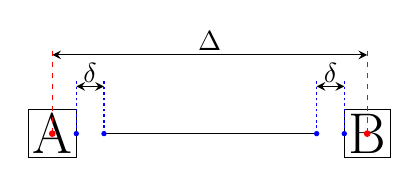
\begin{tikzpicture}[%
    every node/.style={%
      anchor=base,inner sep=1.5pt,outer sep=0pt,minimum size=0pt},
    baseline
    ]
    \node[draw] at(0,0)(aa){\huge A};
    \node[draw]at(4,0)(bb){\huge B};
    \path[shorten <=10pt,shorten >=10pt,draw]
    (aa)--(bb)coordinate[pos=0](al) coordinate[pos=1](bl);
    \node[draw,circle,fill,blue,minimum size=1.5pt,inner sep=0pt]at(al){};
    \node[draw,circle,fill,blue,minimum size=1.5pt,inner sep=0pt]at([xshift=10pt]al){};
    \node[draw,circle,fill,blue,minimum size=1.5pt,inner sep=0pt]at(bl){};
    \node[draw,circle,fill,blue,minimum size=1.5pt,inner sep=0pt]at([xshift=-10pt]bl){};
    \draw[blue,dash pattern=on 1pt off 1pt](bl)--([yshift=0.7cm]bl);
    \draw[blue,dash pattern=on 1pt off 1pt]
    ([xshift=-10pt]bl)--([xshift=-10pt,yshift=0.7cm]bl);
    \draw[stealth-stealth]
    ([yshift=0.6cm]bl.center)--([xshift=-10pt,yshift=0.6cm]bl.center)
    node [midway,above,draw=none]{$\delta$};
    \draw[blue,dash pattern=on 1pt off 1pt](al)--([yshift=0.7cm]al);
    \draw[blue,dash pattern=on 1pt off 1pt]
    ([xshift=10pt]al)--([xshift=10pt,yshift=0.7cm]al);
    \draw[stealth-stealth]
    ([yshift=0.6cm]al.center)--([xshift=10pt,yshift=0.6cm]al.center)
    node [midway,above,draw=none]{$\delta$};
    \node[draw,circle,fill,red,minimum size=2pt,inner sep=0pt]at(aa){};
    \node[draw,circle,fill,red,minimum size=2pt,inner sep=0pt]at(bb){};
    \draw[stealth-stealth]
    ([yshift=1cm]aa.center)--([yshift=1cm]bb.center)
    node [midway,above,draw=none] {$\Delta$};
    \draw[red,dash pattern=on 2pt off2pt](aa.center)--([yshift=1.1cm]aa.center);
    \draw[red,dash pattern=on 2pt off2pt](bb.center)--([yshift=1.1cm]bb.center);
  \end{tikzpicture}
\end{center}

\subsection{Ejemplos con "\texttt{atom sep}", "\texttt{bond offset}"
  y "\texttt{bond style}"}
Estudiaremos tres claves del comando \texttt{\textbackslash chemfig}, relacionadas con
los enlaces:
\begin{itemize}
\item \texttt{atom sep}:
  
  \vspace{-1ex}
  Separación entre los centros de las cajas de los átomos:
  
  \begin{tabular}{|c|c|}\hline
    \vphantom{\rule{0.4pt}{3ex}}
    \chemfig[atom sep=2em]{A-B}
    & \chemfig[atom sep=50pt]{A-B}\\
    \texttt{[\ttres{atom sep=2em}]} & \texttt{[\ttres{atom sep=50pt}]}\\
    \texttt{\textbackslash chemfig\{A-B\}}
    & \texttt{\textbackslash chemfig\{A-B\}}\\
    \hline
  \end{tabular}
  \vspace{1ex}

\item \texttt{bond offset}:
  
  \vspace{-1ex}
  Separación entre borde de caja de átomo y principio del dibujo del enlace.
  
  \begin{tabular}{|c|c|}\hline
    \vphantom{\rule{0.4pt}{3ex}}
    \chemfig[bond offset=0pt]{A-B}
    & \chemfig[bond offset=5pt]{A-B}\\
    \texttt{[\ttres{bond offset=0pt}]} & \texttt{[\ttres{bond offset=5pt}]}\\
    \texttt{\textbackslash chemfig\{A-B\}}
    & \texttt{\textbackslash chemfig\{A-B\}}\\
    \hline
  \end{tabular}
  \vspace{1ex}
  
  Estas claves son globales a la fórmula y se utilizan para toda ella.
  Si quisiéramos aplicar un espacio de separación diferente para un enlace determinado
  en una fórmula, se debería añadir \texttt{\#} justo después del enlace.
  
  \vspace{1ex}
  En adelante, cuando interese, evitaremos escribir el comando
  \texttt{\textbackslash chemfig}, aunque sí escribir los corchetes o llaves que le
  siguen con el fin de disminuir la anchura de las celdas de las tablas en los ejemplos.
  Por el mismo motivo, si hubiera corchetes con opciones generales para la fórmula, se
  pondrían en una línea diferente.

  Si además, se especificara un valor global por defecto para la fórmula, aparecería
  entre corchetes en la primera línea, como en los ejemplos siguientes utiliza una
  distancia, entre borde de la caja y el inicio del dibujo del enlace, de $6pt$.

  \vspace{1ex}
  Si quisiéramos aplicar un espacio de separación diferente para un enlace determinado en
  una fórmula, se añadiría \texttt{\#} justo después del enlace, seguido de un par de
  distancias entre paréntesis y separadas por coma. Estas dos distancias indican el
  espacio entre el borde de la caja del primer átomo hasta que se dibuja el enlace, y la
  segundo es el espacio entre el final del enlace y el comienzo de la caja del segundo
  átomo. Si no se especifica alguna de las distancias, se asumiría el valor por defecto.
  
  \vspace{1ex}
  En el siguiente ejemplo se considera un valor de espaciado \emph{átomo--enlace} de
  \texttt{6pt}, lo que se refleja en la primera línea de la tabla.
  
  En la fórmula de la izquierda, el primer enlace tiene un espaciado de $0pt$ al
  principio y al final. En la segunda especificamos que el segundo enlace tenga un
  espaciado de $2pt$ al final de este. En la tercera indicamos un espaciado de $2pt$ al
  principio; cuando no se especifica nada para un enlace, se utilizan los \texttt{6pt}:
  
    \setchemfig{bond offset=6pt}
    \begin{tabular}{|c|c|c|}\hline
      \multicolumn{3}{|c|}{%
      {\large\texttt{\textbackslash setchemfig\{bond offset=6pt\}}}
      }\\\hline
      \vphantom{$\dfrac{1}{1}$}
      \chemfig{A-#(0pt,0pt)B-C}
      & \chemfig{A-B-#(,2pt)C}
      & \chemfig{A-B-#(2pt)C}\\
      \texttt{\{A-\ttres{\#(0pt,0pt)}B-C\}}
      & \texttt{\{A-B-\ttres{\#(,2pt)}C\}}
      & \texttt{\{A-B-\ttres{\#(2pt)}C\}}\\
      \hline
    \end{tabular}

  Por ejemplo, la fórmula de la izquierda se escribiría como
  \begin{center}
    \texttt{\textbackslash chemfig[bond offset=0pt]\{A-\#(0pt,0pt)B-C\}}
  \end{center}

  \vspace{1ex}
\item \texttt{bond style}:

  \vspace{-1ex}
  A los enlaces de la fórmula se le aplican los estilos del paquete de dibujo
  \textsf{TikZ}:

  \begin{tabular}{|c|}\hline
    \vphantom{\rule{0.4pt}{3ex}}
    \chemfig[bond style={line width=1pt,Red}]{A>|B-C<:D}\\
    \texttt{[\ttres{bond style=\{line width=1pt,red\}}]}\\
    \texttt{\{A>|B=C-D<:E\}}\\
    \hline
  \end{tabular}
%\end{itemize}

  \begin{tabular}{|c|}\hline
    \vphantom{\rule{0.4pt}{3ex}}
    \chemfig[bond style={line width=1pt,dotted,red}]{A-B}\\
    \texttt{[\ttres{bond style=\{line width=1pt,dotted,red\}}]}\\  
    \texttt{\{A-B\}}\\
    \hline
  \end{tabular}
\end{itemize}

\subsection{Ángulos en los enlaces}
Hasta ahora hemos dispuesto los enlaces horizontalmente, formando un ángulo de
\qty{0}{\degree} medido desde el átomo de partida. Si no se especifica nada, este
es el ángulo por defecto, pero podemos cambiarlo.

Hay varias formas de especificar los ángulos:
\begin{itemize}
\item Por múltiplos de \qty{45}{\degree}, o lo que indique el parámetro
  \texttt{angle increment}:

  \vspace{-1ex}
  En este caso, este indica el múltiplo de \qty{45}{\degree} que forma el ángulo con
  respecto del átomo de partida. Este número se escribe entre corchetes:

  \begin{tabular}{|c|c|c|c|}\hline
    \vphantom{\rule{0.4pt}{10ex}}
    \chemfig{A-B}
    & \chemfig{A-[1]B}
    & \chemfig{A-[2]B}
    & \chemfig{A-[3]B}\\
    {\footnotesize\texttt{\{A-B\}}}
    & {\footnotesize\texttt{\{A-\ttres{[1]}B\}}}
    & {\footnotesize\texttt{\{A-\ttres{[2]}B\}}}
    & {\footnotesize\texttt{\{A-\ttres{[3]}B\}}}\\
    $\ttres{0}\cdot\qty{45}{\degree} = \qty{0}{\degree}$
    & {\small $\ttres{1}\cdot\qty{45}{\degree} = \qty{45}{\degree}$}
    & {\small $\ttres{2}cdot\qty{45}{\degree} = \qty{90}{\degree}$}
    & {\small $\ttres{3}\cdot\qty{45}{\degree} = \qty{135}{\degree}$}
    \\\hline
  \end{tabular}

  \begin{tabular}{|c|c|c|c|}\hline
    \vphantom{\rule{0.4pt}{3ex}}
    \chemfig{A-[4]B}
    & \chemfig{A-[5]B}
    & \chemfig{A-[6]B}
    & \chemfig{A-[7]B}\\
    \texttt{\{A-\ttres{[4]}B\}}
    & \texttt{\{A-\ttres{[5]}B\}}
    & \texttt{\{A-\ttres{[6]}B\}}
    & \texttt{\{A-\ttres{[7]}B\}}\\
    {\small $\ttres{4}\cdot\qty{45}{\degree} = \qty{180}{\degree}$}
    & {\small $\ttres{5}\cdot\qty{45}{\degree} = \cdots = \qty{-135}{\degree}$}
    & {\small $\ttres{6}\cdot\qty{45}{\degree} = \cdots = \qty{-90}{\degree}$}
    & {\small $\ttres{7}\cdot\qty{45}{\degree} = \cdots = \qty{-45}{\degree}$}
    \\\hline
  \end{tabular}
  \vspace{1ex}

\item Ángulos absolutos:

  \vspace{-1ex}
  El ángulo absoluto se escribe entre corchetes precedido de dos puntos.
  
  Ejemplos:

  \begin{tabular}{|c|}\hline
    \vphantom{\rule{0.4pt}{5ex}}
    \chemfig{A-B-[:-45]C-D-[:90]E}\\
    \vphantom{\rule{0.4pt}{3ex}}
    \texttt{[atom sep=2em]}\\
    \{A-B-\ttres{[:-45]}C-D-\ttres{[:90]}E\}\\
    \hline
  \end{tabular}

  \begin{tabular}{|c|c|}\hline
    \vphantom{\rule{0.4pt}{5ex}}
    \chemfig[atom sep=2em]{-[:30]-[:-30]-[:-90]-[:-150]-[:150]-[:90]}\\
    \texttt{[atom sep=2em]}\\ \{-\ttres{[:30]}-\ttres{[:-30]}-\ttres{[:-90]}-\ttres{[:-150]}-\ttres{[:150]}-\ttres{[:90]}\}\\
    \hline
  \end{tabular}

\item Ángulos relativos:

  \vspace{-1ex}
  El ángulo relativo de un enlace, con respecto al anterior, se escribe entre corchetes
  precedido de doble carácter de dos puntos. El primer ángulo debe ser absoluto.
  
  Ejemplos:

  \begin{tabular}{|c|}\hline
    \vphantom{\rule{0.4pt}{8ex}}
    \chemfig[atom sep=3em]{A-B-[::-45]C=[::135]D}\\
    \vphantom{\rule{0.4pt}{3ex}}
    \texttt{[atom sep=3em]}\\
    \texttt{\{A-B-\ttres{[::-45]}C=\ttres{[::135]}D\}}\\
    \hline
  \end{tabular}

  \begin{tabular}{|c|}\hline
    \vphantom{\rule{0.4pt}{8ex}}
    \chemfig[atom sep=3em]{-[:36]-[::-72]-[::-72]-[::-72]-[::-72]}\\
    \vphantom{\rule{0.4pt}{3ex}}
    \texttt{[atom sep=3em]}\\
    \texttt{\{-[:-36]-\ttres{[::-72]}-\ttres{[::-72]}-\ttres{[::-72]}-\ttres{[::-72]}\}}\\
    \hline
  \end{tabular}
  
\end{itemize}


\subsection{Longitud de los enlaces}
Vimos anteriormente que, en lugar de longitud de enlace, deberíamos hablar de espaciado
interatómico (distancia entre los centros de las cajas, \texttt{atom sep}).
Este espaciado es el que tiene en cuenta por defecto y siempre que
\texttt{fixed length=false}. De esta manera \textsf{chemfig} utiliza un espaciado
interatómico fijo y la longitud de enlace se amolda a ello y al valor de
\texttt{bond offset} (imagen de la izquierda).

En cambio, si \texttt{fixed length=true}, entonces \texttt{atom sep} se interpreta como
distancia mínima entre los bordes de las cajas de los átomos que se unen (imagen de la
derecha).

\begin{center}
  \begin{tabular}{c@{\kern1.50cm}c}
    \CFkv{fixed length}{false}&\CFkv{fixed length}{true}\\[2ex]
    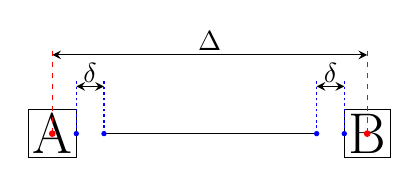
\begin{tikzpicture}[%
      every node/.style={anchor=base,inner sep=1.5pt,outer sep=0pt, minimum size=0pt},
      baseline
      ]
      \node[draw] at(0,0)(aa){\huge A};
      \node[draw]at(4,0)(bb){\huge B};
      \path[shorten <=10pt,shorten >=10pt,draw]
      (aa)--(bb)coordinate[pos=0](al) coordinate[pos=1](bl);
      \node[draw,circle,fill,blue,minimum size=1.5pt,inner sep=0pt]at(al){};
      \node[draw,circle,fill,blue,minimum size=1.5pt,inner sep=0pt]
      at([xshift=10pt]al){};
      \node[draw,circle,fill,blue,minimum size=1.5pt,inner sep=0pt]at(bl){};
      \node[draw,circle,fill,blue,minimum size=1.5pt,inner sep=0pt]
      at([xshift=-10pt]bl){};
      \draw[blue,dash pattern=on 1pt off 1pt](bl)--([yshift=0.7cm]bl);
      \draw[blue,dash pattern=on 1pt off 1pt]
      ([xshift=-10pt]bl)--([xshift=-10pt,yshift=0.7cm]bl);
      \draw[stealth-stealth]
      ([yshift=0.6cm]bl.center)--([xshift=-10pt,yshift=0.6cm]bl.center)
      node [midway,above,draw=none]{$\delta$};
      \draw[blue,dash pattern=on 1pt off 1pt](al)--([yshift=0.7cm]al);
      \draw[blue,dash pattern=on 1pt off 1pt]
      ([xshift=10pt]al)--([xshift=10pt,yshift=0.7cm]al);
      \draw[stealth-stealth]
      ([yshift=0.6cm]al.center)--([xshift=10pt,yshift=0.6cm]al.center)
      node [midway,above,draw=none]{$\delta$};
      \node[draw,circle,fill,red,minimum size=2pt,inner sep=0pt]at(aa){};
      \node[draw,circle,fill,red,minimum size=2pt,inner sep=0pt]at(bb){};
      \draw[stealth-stealth]
      ([yshift=1cm]aa.center)--([yshift=1cm]bb.center)
      node [midway,above,draw=none] {$\Delta$} ;
      \draw[red,dash pattern=on 2pt off2pt](aa.center)--([yshift=1.1cm]aa.center);
      \draw[red,dash pattern=on 2pt off2pt](bb.center)--([yshift=1.1cm]bb.center);
    \end{tikzpicture}
  &
    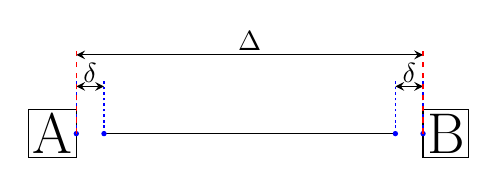
\begin{tikzpicture}[%
      every node/.style={anchor=base,inner sep=1.5pt,outer sep=0pt,minimum size=0pt},
      baseline]
      \node[draw] at(0,0)(aa){\huge A};
      \node[draw]at(5,0)(bb){\huge B};
      \path[shorten <=10pt,shorten >=10pt,draw]
      (aa)--(bb)coordinate[pos=0](al) coordinate[pos=1](bl);
      \node[draw,circle,fill,blue,minimum size=1.5pt,inner sep=0pt]at(al){};
      \node[draw,circle,fill,blue,minimum size=1.5pt,inner sep=0pt]
      at([xshift=10pt]al){};
      \node[draw,circle,fill,blue,minimum size=1.5pt,inner sep=0pt]at(bl){};
      \node[draw,circle,fill,blue,minimum size=1.5pt,inner sep=0pt]
      at([xshift=-10pt]bl){};
      \draw[blue,dash pattern=on 1pt off 1pt](bl)--([yshift=0.7cm]bl);
      \draw[blue,dash pattern=on 1pt off 1pt]
      ([xshift=-10pt]bl)--([xshift=-10pt,yshift=0.7cm]bl);
      \draw[stealth-stealth]
      ([yshift=0.6cm]bl.center)--([xshift=-10pt,yshift=0.6cm]bl.center)
      node [midway,above,draw=none]{$\delta$};
      \draw[blue,dash pattern=on 1pt off 1pt](al)--([yshift=0.7cm]al);
      \draw[blue,dash pattern=on 1pt off 1pt]
      ([xshift=10pt]al)--([xshift=10pt,yshift=0.7cm]al);
      \draw[stealth-stealth]
      ([yshift=0.6cm]al.center)--([xshift=10pt,yshift=0.6cm]al.center)
      node [midway,above,draw=none]{$\delta$};
      \draw[stealth-stealth]([yshift=1cm]al)--([yshift=1cm]bl)
      node [midway,above,draw=none] {$\Delta$} ;
      \draw[red,dash pattern=on 2pt off2pt](al)--([yshift=1.1cm]al);
      \draw[red,dash pattern=on 2pt off2pt](bl)--([yshift=1.1cm]bl);
    \end{tikzpicture}
  \end{tabular}
\end{center}

\vspace{1ex}
En el siguiente ejemplo, los átomos en la molécula de yodo entre sí y los de \ce{H3} con
\ce{C}, están situados a la misma distancia y, como consecuencia, la longitud de enlace
es diferente:

\begin{tabular}{|c|c|}\hline
  \multicolumn{2}{|c|}{\ttres{fixed length=false}}\\\hline
  \vphantom{\rule{0.4pt}{3ex}}
  \chemfig{I-I}
  & \chemfig{CH_3-CH_3}\\
  \texttt{\textbackslash chemfig\{I-I\}}
  & \texttt{\textbackslash chemfig\{CH\_3-CH\_3\}}\\\hline
\end{tabular}

\vspace{1ex}
Comparamos el resultado de los comandos anteriores, situando las dos fórmulas en filas
diferentes y observamos que las distancias entre los centros de las cajas es la misma:

\begin{center}
  \begin{tabular}{|c|}\hline
    \vphantom{\rule{0.4pt}{3ex}}
    \chemfig{I-I}\\
    \chemfig{CH_3-CH_3}\\[1ex]
    \hline
  \end{tabular}
\end{center}

Pero, cuando indicamos \texttt{fixed length=true}, la longitud de enlace es relativamente
constante, aunque depende además, de la inclinación del enlace y del tamaño del átomo.
Para la longitud del enlace se toma la distancia definida en \texttt{atom sep=<dim>}:

\begin{tabular}{|c|c|}\hline
  \multicolumn{2}{|c|}{\ttres{fixed length=true}}\\\hline
  \vphantom{\rule{0.4pt}{3ex}}
  \chemfig[fixed length=true]{I-I}
  & \chemfig[fixed length=true]{CH_3-CH_3}\\
  \texttt{\textbackslash chemfig\{I-I\}}
  & \texttt{\textbackslash chemfig\{CH\_3-CH\_3\}}\\\hline
\end{tabular}

\vspace{1ex}
Comparamos de nuevo las dos fórmulas y vemos que ahora la distancia entre los bordes
de las cajas es la misma, y si \texttt{bond offset} es idéntico en ambas, como en
el ejemplo, el enlace tiene la misma longitud:

\begin{center}
  \begin{tabular}{|c|}\hline
    \vphantom{\rule{0.4pt}{3ex}}
    \chemfig[fixed length=true]{I-I}\\
    \chemfig[fixed length=true]{CH_3-CH_3}\\[1ex]
    \hline
\end{tabular}
\end{center}

\vspace{1ex}
Incluso con \texttt{fixed length=true}, cuando los átomos se encuentran en un ciclo,
no se respeta tal condición, sino que se da prioridad a la distancia interatómica
constante, para que el ciclo sea regular, siempre que se pueda.

En algunas situaciones, especialmente, cuando \textsf{chemfig} tiene el comportamiento
por defecto (\texttt{fixed length=false}), pueden formarse enlaces muy cortos y se
necesitaría aumentar (o disminuir) la distancia interatómica en algún enlace concreto.
Para ello, no vale \texttt{\textbackslash chemfig[atom sep=valor]\{...\}}, porque
afectaría a todos los enlaces de la molécula.

Se puede indicar esa distancia en un enlace concreto añadiendo argumentos entre
corchetes. Ya vimos que el primer argumento indicaba el ángulo que formaba el enlace.
Un segundo argumento, separado del primero por una coma, indica la distancia
interatómica. Este argumento es un número entero positivo, que indica el factor por
el que se multiplica la distancia interatómica.

En el ejemplo de la izquierda, el primer átomo, \ce{A_2^{2+}}, es muy ancho y el centro
de su caja provoca que el enlace sea muy corto, que se ve en la figura de la izquierda.

En el ejemplo de la derecha, el enlace sencillo viene acompañado del corchete
\texttt{[,2]}. El primer argumento está vacío, por lo que se utilizará para el enlace el
ángulo por defecto, \qty{0}{\degree}. El segundo argumento es un $2$, lo que indica que
la distancia interatómica para ese enlace es el doble de la especificada en
\texttt{atom sep}.

\begin{tabular}{|c|c|}\hline
  \multicolumn{2}{|c|}{\texttt{fixed length=false}}\\\hline  
  \vphantom{\rule{0.4pt}{3ex}}
  \chemfig{{A_2}^{2+}-B_3}
  & \chemfig{{A_2}^{2+}-[,2]B_3}\\
  \texttt{\{\{A\_2\}\textasciicircum\{2+\}-B\_3\}}
  & \texttt{\{A\_2\}\textasciicircum\{2+\}-\ttres{[,2]}B\_3\}}\\\hline
\end{tabular}

\subsection{Tamaño de las fórmulas}
Podemos cambiar el tamaño de las moléculas cambiando el tamaño de la fuente, los
enlaces se escalan de forma apropiada si \texttt{atom sep} se ha definido en función
de la fuente, por ejemplo \text{em} o \text{ex}. Porque estas unidades dependen de
la fuente elegida.

\begin{tabular}{|c|c|}\hline
  \vphantom{\rule{0.4pt}{7ex}}
  \chemfig{H-[:37]O-[::-72]H}
  & {\small\chemfig{H-[:37]O-[::-72]H}}\\
  {\small\texttt{\textbackslash chemfig\{\{H-[:37]O-[::-72]H\}\}}}
  & {\small\texttt{\ttres{\{\textbackslash small}\textbackslash chemfig\{\{H-[:37]O-[::-72]H\}\}}\ttres{\}}}\\
  \hline
\end{tabular}


\subsection{Átomos de salida y llegada}
Un grupo de átomos suele estar formado por varios átomos, como \ce{CH3}, que está
formado por los \emph{átomos} \ce{C} y \ce{H3}. Supongamos que nos interesa unir
mediante enlaces dos grupos de átomos, digamos \ce{ABCD} y \ce{EFG}. Por defecto,
\textsf{chemfig} intentará unir los átomos que tenga más cerca dependiendo del ángulo que
se especifique.

En el ejemplo de la izquierda, el enlace une los átomos más cercanos \ce{C} y \ce{D}.
En el centro, se unen \ce{C} y \ce{D}. A la derecha se unen \ce{A} y \ce{F}:

\begin{tabular}{|c|c|c|}\hline
  \vphantom{\rule{0.4pt}{6ex}}
  \chemfig{ABC-DEF}
  & \chemfig{ABC-[:30]DEF}
  & \chemfig{ABC-[:150]DEF}\\
  \texttt{\{ABC-DEF\}\}}
  &\texttt{\{ABC-[:30]DEF\}\}}
  & \texttt{\{ABC-[:150]DEF\}\}}\\
  \hline
\end{tabular}

\vspace{1ex}
¿Cómo podríamos obligar a \textsf{chemfig} a unir átomos distintos a los que elige por
defecto?
Ya hemos visto dos argumentos para modificar un  enlace particular, el primero era el
ángulo del enlace, el segundo es el factor que afecta a \texttt{atom sep}, el tercero
indica el átomo desde el que sale el enlace y el cuarto el átomo al que llega.
Los átomos de salida y llegada se indican mediante números naturales:
\begin{center}
  {\small
    \texttt{"enlace"%
      [ángulo, distancia entre átomos, \emph{átomo de salida}, \emph{átomo de
        llegada]}
    }
  }
\end{center}

En el ejemplo de la izquierda, se unen por defecto los átomos \ce{C} y \ce{D} por que
se encuentran más cerca entre sí; en cambio, a la derecha obligamos a que el primer átomo
de cada uno de los grupos sean los que se enlacen:
 
\begin{tabular}{|c|c|}\hline
  \vphantom{\rule{0.4pt}{10ex}}
  \chemfig{ABC-[:60]DEF}
  & \chemfig{ABC-[:60,,1,1]DEF}\\
  \texttt{\{ABC-[:60]DEF\}\}}
  & \texttt{\{ABC-[:60\ttres{,,1,1}]DEF\}}\\\hline
\end{tabular}

\vspace{1ex}
Otro ejemplo:

\begin{tabular}{|c|c|}\hline
  \vphantom{\rule{0.4pt}{10ex}}
  \chemfig{ABC-[:135]DEF}
  & \chemfig{ABC-[3,,2,3]DEF}\\
  \texttt{\{ABC-[:135]DEF\}}
  & \texttt{\{ABC-[3\ttres{,,2,3}]DEF\}}\\\hline
\end{tabular}

Por supuesto, 3 en el parámetro de ángulo de enlace es equivalente a un ángulo de
\qty{135}{\degree}, siempre que \texttt{angle increment=45}.

\subsection{Personalización mediante \textsf{TikZ}}
Hay un quinto argumento para personalizar un enlace: \texttt{[,,,,<\textsf{TikZ}>]}.
Veamos unos ejemplos:

\begin{tabular}{|cl|}\hline
  \vphantom{\rule{0.4pt}{3ex}}
  \chemfig{A-[,,,,line width=1.4pt,red]B}
  & \texttt{\{A-[,,,,line width=1.2pt,red]B\}}\\\hline
  \vphantom{\rule{0.4pt}{3ex}}
  \chemfig{A-[,,,,line width=0.8pt,dash pattern=on 2pt off 2pt,blue]B}
  & {\small
    \texttt{\{A-[,,,,line width=0.8pt,dash pattern=on 2pt off 2pt]B\}}}\\\hline
  \vphantom{\rule{0.4pt}{3ex}}
  \chemfig{A-[,1.5,,,decorate,decoration=snake]B}
  & \texttt{\{A-[,2,,,decorate,decoration=snake]B\}}\\\hline
  \vphantom{\rule{0.4pt}{3ex}}
  \chemfig{A-[,1.4,,,decorate,decoration=coil,segment length=0.3em]B}
  & {\footnotesize
    \texttt{\{A-[,1.4,,,decorate,decoration=coil,segment length=0.3em]B\}}}\\\hline
\end{tabular}


\subsection{Conectando enlaces}
Cuando se unen enlaces entre sí, no se ajustan perfectamente, sobre todo esto es
visible cuando el grosor del enlace es grande. Para que se unan perfectamente hay que
añadir \texttt{bond join=true} o simplemente \texttt{bond join}.

Veamos los siguientes ejemplos. En el primero unimos los dos enlaces y parece que todo
está bien. En el segundo ampliamos el grosor de las líneas y comprobamos que no forman
una unión completa. En el tercero, añadimos \texttt{bond join=true}, utilizando una
anchura de línea grande y comprobamos que la unión forma un vértice perfecto. En el
cuarto, utilizamos el grosor por defecto del enlace, e incluso escribimos
\texttt{bond join}, sin el \texttt{=true}:

\begin{tabular}{|cl|}\hline
  \vphantom{\rule{0.4pt}{6ex}}
  \chemfig{-[:45]-[::-90]}
  & \texttt{\textbackslash chemfig\{-[:45]-[::-90]\}}\\\hline
  \vphantom{\rule{0.4pt}{6ex}}
  \chemfig[bond style={line width=3.5pt}]{-[:45]-[::-90]}
  & \texttt{[bond style=\{line width=3.5pt\}]\{-[:45]-[::-90]\}}\\\hline
  \vphantom{\rule{0.4pt}{6ex}}
  \chemfig[\ttres{bond join=true},bond style={line width=3.5pt}]{-[:45]-[::-90]}
  & {\footnotesize
    \texttt{[\ttres{bond join=true},bond style=\{line width=3.5pt\}]\{-[:45]-[::-90]\}}}\\\hline
  \vphantom{\rule{0.4pt}{6ex}}
  \chemfig[bond join]{-[:45]-[::-90]}
  & \texttt{[bond join]\{-[:45]-[::-90]\}}\\\hline
\end{tabular}


\subsection{Valores por defecto para los enlaces}
Las propiedades de los enlaces están determinadas por cinco parámetros:
\begin{center}
  \texttt{[ángulo, coeficiente, salida, llegada, TikZ]}
\end{center}

Por defecto, \textsf{chemfig} utiliza los siguientes valores:
\begin{enumerate}
\item Primera posición, ángulo: \qty{0}{\degree}

  \vspace{-1ex}
  El enlace se dirige de izquierda a derecha.
  
\item Segunda posición, coeficiente: 1

  \vspace{-1ex}
  La distancia entre los átomos o la longitud del enlace es
  1 multiplicado por la distancia especificada para \texttt{atom sep} (dependiendo del
  valor de \texttt{fixed length}).
  
\item Tercer y cuarta posiciones, átomos de salida y llegada: \rule[0.5ex]{1.5em}{0.6pt}

  \vspace{-1ex}
  Lo que indica que el enlace se dirige
  entre los dos átomos más cercanos, teniendo en cuenta el ángulo que forma el enlace.
  
\item Quinta posición, estilo TikZ: \rule[0.5ex]{1.5em}{0.6pt}

  \vspace{-1ex}
  No añade ningún estilo especial de \textsf{TikZ}.
\end{enumerate}

\vspace{1ex}
Podemos modificar estos valores, especificando entre corchetes los valores que queremos
cambiar, respetando el orden de las comas:
\begin{itemize}
\item Para un enlace concreto de una molécula, justo después del enlace.  
\item Para todos los enlaces de una molécula en particular, al principio del comando
  \texttt{\textbackslash chemfig}, justo después de la llave de apertura "\texttt{\{}".
\end{itemize}

\vspace{1ex}
En el primer ejemplo, especificamos un ángulo de enlace, distancia interatómica y color
para el enlace entre \ce{A} y \ce{B}, que no afecta al segundo enlace, entre \ce{B} y
\ce{C}.

\begin{tabular}{|cl|}\hline
  \vphantom{\rule{0.4pt}{6ex}}
  \chemfig{A-[:15,2,,,,red]B-C}
  & \texttt{\textbackslash chemfig\{A-\ttres{[:15,2,,,,red]}B-C\}}\\
  \hline
\end{tabular}

\vspace{1ex}
En el segundo ejemplo, definimos color rojo para los enlaces de la molécula al principio
del comando, por lo que afectará a todos los enlaces, excepto a los enlaces que se
cambien explícitamente. En este ejemplo, para el doble enlace indicamos color verde y el
último enlace vuelve a ser rojo, como habíamos indicado por defecto en esta molécula:
    
\begin{tabular}{|cl|}\hline
  \vphantom{\rule{0.4pt}{3ex}}
  \chemfig{[,,,,red]A-B=[,,,,green]C-D}
  & \texttt{\textbackslash chemfig\{\ttres{[,,,,red]}A-B=\ttresg{[,,,,green]}C-D\}}\\[0.5ex]
  \hline
\end{tabular}

\vspace{1ex}
En el tercer ejemplo, definimos un ángulo de enlace absoluto de \qty{15}{\degree} y una distancia interatómica un \qty{75}{\percent} para toda la fórmula:

\begin{tabular}{|c|c|}\hline
  \vphantom{\rule{0.4pt}{6.5ex}}
  \chemfig{A-B-C}
  & \chemfig{[:15,0.75]A-B-C}\\
  \texttt{\textbackslash chemfig\{A-B-C\}}
  & \texttt{\textbackslash chemfig\{\ttres{[:15,0.75]}A-B-C\}}\\
  \hline
\end{tabular}

\subsection{Ramificaciones}
Hasta ahora, las fórmulas las hemos escrito de forma que los grupos de átomos se unían
en línea, unos después de otros, formando una cadena abierta horizontal, vertical,
formando un cierto ángulo o una línea quebrada.

Pero se pueden añadir \emph{ramificaciones} a las cadenas anteriores (esto también
servirá para las ramificaciones en los ciclos, cuando los veamos).
¿Cómo se añaden estas? Insertando entre paréntesis, justo después del átomo que sufre la
ramificación un enlace, posibles parámetros que le afecten y los átomos involucrados.

En el primer ejemplo representamos una cadena lineal genérica \ce{A-B-C}.
A su derecha añadimos en el segundo átomo de la cadena, la ramificación
\texttt{-[2]W-X}, que se encierra entre paréntesis (recordemos que el número 2, como
primer parámetro indica que la ramificación forma un ángulo absoluto de
$2\cdot\qty{45}{\degree}=\qty{90}{\degree}$.

\begin{tabular}{|c|c|}\hline
  \vphantom{\rule{0.4pt}{10ex}}
  \chemfig{A-B-C}
  & \chemfig{A-B(-[2,,,,red]\ttres{W}-[,,,,red]\ttres{X})-C}\\
  \texttt{\{A-B-C\}}
  & \texttt{\{A-B\ttres{(-[2]W-X)}-C\}}\\
  \hline
\end{tabular}

donde la ramificación se ha señalado en rojo.

\vspace{1ex}
Se recomienda escribir el código de la cadena base que nos interesa, y cuando comprobemos
que produce la estructura correcta, entonces insertar paréntesis de apertura y cierre
después del átomo que sufre la ramificación y, por último completar esta.

Aunque la fórmula anterior se ha escrito y se lee fácilmente, suele ser recomendable
dibujar la estructura base (que no necesariamente la cadena principal tal y como se
define en formulación orgánica, pues aquí no nos importan los enlaces múltiples, entre
otras cosas) que tenga más átomos, y el resto como ramificaciones; deesta forma
disminuimos el número de ellas o la longitud de estas, que son situaciones que en
fórmulas complejas pueden complicar la lectura del código fuente.

Según este criterio, la fórmula anterior se podría haber escrito de varias formas;
una de ellas es representar la estructura base de cuatro átomos
\ce{A-B-W-X}, y añadir como ramificación la \ce{C}. De nuevo se señala la ramificación
en rojo:

\begin{tabular}{|c|c|}\hline
  \vphantom{\rule{0.4pt}{10ex}}
  \chemfig{A-B-[2]W-X}
  & \chemfig{A-B(-[,,,,red]\ttres{C})-[2]W-X}\\
  \texttt{%
  \textbackslash chemfig\{A-B-[2]W-X\}
  }
  & \texttt{%
    \textbackslash chemfig\{%
    \{A-B\ttres{(-C)}-[2]W-X}\\\hline
\end{tabular}


\section{Configuración por defecto}
A partir de ahora utilizaremos un sistema de valores por defecto para \textsf{chemfig}.
Estos valores pueden variar según las preferencias del usuario. En todo caso, tómese
como una propuesta.

Esta configuración propone unas distancias interatómicas más cortas entre otras
cosas. Es conveniente añadir estos valores u otros, según interese, en el preambulo del
documento\footnotemark{}:
\footnotetext{Para este documento no lo he puesto en el preámbulo porque hasta aquí he
  preferido mostrar la configuración por defecto de \textsf{chemfig}; la añado en
  este punto concreto del documento para que se aplique en adelante.}

\texttt{%
\noindent\textbackslash setchemfig\{\\
\hspace*{2em}atom sep=2.0em, {\small\% Reduce la longitud de los enlaces}\\
\hspace*{2em}bond offset=2pt, {\small\% Espacio entre el átomo y el inicio del enlace}\\
\hspace*{2em}double bond sep=2.5pt, {\footnotesize\% Espacio entre líneas de un enlace múltiple}\\
\hspace*{2em}bond spacing=3.0pt, {\small\% Espacio reservado para los enlaces múltiples}\\
\hspace*{2em}cram size=3pt, {\footnotesize\% Ancho de la base de los enlaces de tipo Cram (cuñas)}\\
\hspace*{2em}node style=\{scale=0.85\} {\small\% Escala las etiquetas de los átomos}\\
\}}


\setchemfig{
  atom sep = 1.8em,       % Reduce la longitud de los enlaces (por defecto es 3.0em)
  bond offset = 1.6pt,      % Espacio entre el átomo y el inicio del enlace
  double bond sep = 2.5pt,% Espacio entre las dos líneas de un enlace doble
  bond spacing = 3.0pt,   % Espacio entre los puntos de un par solitario (Lewis)
  cram size = 3pt,        % Ancho de la base de los enlaces de tipo Cram (cuñas)
  node style = {scale=0.85} % Escala ligeramente las etiquetas de los átomos
}

A partir de ahora se aplicarán los valores anteriores por defecto, a menos que se diga
lo contrario.

\section{Línea base}
El primer elemento, átomo o enlace que se dibuja en una fórmula define la línea base,
que se indica en rojo.

En este ejemplo, el átomo \ce{A} es el primero que aparece en el comando
\texttt{\textbackslash chemfig} y, por tanto, define la línea base:

\begin{tabular}{|l|}\hline
  \vphantom{\rule{0.4pt}{2.5ex}}
  \vphantom{\chemfig{A-B}}\tikz \draw[help lines, red,] (0,0) -- (5em,0);
  \chemfig{A-B}
  \tikz \draw[help lines, red] (0,0) -- (5em,0);
  \\[0.25ex]
  \multicolumn{1}{|c|}{%
  \vphantom{\rule{0.4pt}{3ex}}
  \texttt{\textbackslash chemfig\{\ttres{A}-B\}}
  }
  \\\hline
\end{tabular}

\vspace{1ex}
Cuando no se representa el átomo que define la línea base, se supone que es un punto
invisible sin tamaño y su linea base es la misma que la del enlace que le sigue:

\begin{tabular}{|c|}\hline
  \vphantom{\rule{0.4pt}{2ex}}
  \vphantom{\chemfig{-B}}\tikz \draw[help lines, red] (0,0) -- (5em,0);
  \chemfig{-B}
  \tikz \draw[help lines, red] (0,0) -- (5em,0);
  \\[0.25ex]
  \vphantom{\rule{0.4pt}{3ex}}
  \texttt{\textbackslash chemfig\{\ttres{-}B\}}
  \\\hline
\end{tabular}

\vspace{1ex}
En la siguiente fórmula hemos puesto \ce{A} como primer átomo:

\begin{tabular}{|c|}\hline
  \vphantom{\rule{0.4pt}{2.5ex}}
  \vphantom{\chemfig{A-[7]B}}\tikz \draw[help lines, red] (0,0) -- (5em,0);
  \chemfig{A-[7]B}
  \tikz \draw[help lines, red] (0,0) -- (5em,0);
  \\[3.5ex]
  \vphantom{\rule{0.4pt}{3ex}}
  \texttt{\textbackslash chemfig\{\ttres{A}-[7]B\}}
  \\\hline
\end{tabular}

\vspace{1ex}
Ahora repetimos la misma fórmula, pero dibujamos primero \ce{B}:

\begin{tabular}{|c|}\hline
  \vphantom{\rule{0.4pt}{6ex}}
  \vphantom{\chemfig{B-[3]A}}\tikz \draw[help lines, red] (0,0) -- (5em,0);
  \chemfig{B-[3]A}
  \tikz \draw[help lines, red] (0,0) -- (5em,0);
  \\[0.25ex]
  \vphantom{\rule{0.4pt}{3ex}}
  \texttt{\textbackslash chemfig\{\ttres{B}-[3]A\}}
  \\\hline
\end{tabular}

\vspace{1ex}
Hemos dicho que el primer átomo define la línea base, pero hay un parámetro que hace que
se sitúe por encima o por debajo del átomo. El parámetro es \texttt{baseline=<dim>}.

En el siguiente ejemplo, la línea base se sitúa $5pt$ por encima de la base del átomo:

\begin{tabular}{|l|}\hline
  \vphantom{\rule{0.4pt}{2ex}}
  \vphantom{\chemfig{A-B}}\tikz \draw[help lines, red,] (0,0) -- (5em,0);
  \chemfig[baseline=5pt]{A-B}
  \tikz \draw[help lines, red] (0,0) -- (5em,0);
  \\[1.25ex]
  \multicolumn{1}{|c|}{%
  \vphantom{\rule{0.4pt}{3ex}}
  \texttt{\textbackslash chemfig[\ttres{baseline=5pt}]\{A-B\}}
  }
  \\\hline
\end{tabular}

\vspace{1ex}
Ahora se sitúa $5pt$ por debajo de la base del átomo:

\begin{tabular}{|l|}\hline
  \vphantom{\rule{0.4pt}{4ex}}
  \vphantom{\chemfig{A-B}}\tikz \draw[help lines, red,] (0,0) -- (5em,0);
  \chemfig[baseline=-5pt]{A-B}
  \tikz \draw[help lines, red] (0,0) -- (5em,0);
  \\[1ex]
  \multicolumn{1}{|c|}{%
  \vphantom{\rule{0.4pt}{3ex}}
  \texttt{\textbackslash chemfig[\ttres{baseline=-5pt}]\{A-B\}}
  }
  \\\hline
\end{tabular}


\section{Ramificaciones en cadenas abiertas}
En los primeros ejemplos que siguen se han señalado en negrita los átomos de carbono
que forman la cadena base (no necesariamente la cadena principal), igual que en el código
se señalan las ramificaciones en rojo.

\subsection{\emph{Isobutano} o metilpropano}
Observa que las dos fórmulas tienen la misma altura porque utilizan la misma línea base, dado que utilizan el mismo átomo \ce{C} en primer lugar:

\begin{tabular}{|c|c|}\hline
  \vphantom{\rule{0.4pt}{7ex}}
  \chemfig{\textbf{C}H_3-\textbf{C}H(-[2]CH_3)-\textbf{C}H_3}
  & \chemfig{\textbf{C}H_3-CH(-[6]CH_3)-CH_3}\\
  \texttt{\{CH\_3-CH\ttres{(-[2]CH\_3)}-CH\_3\}}
  & \texttt{\{CH\_3-CH\ttres{(-[2]CH\_3)}-CH\_3\}}\\
  \hline
\end{tabular}

\vspace{1ex}
A la izquierda, se ha comenzado por el grupo de átomos \ce{CH3} superior.
A la derecha se ha comenzado por el \ce{CH3} más a la izquierda.
Podemos comprobar que ambos grupos de átomos están a la misma altura (misma línea base):

\begin{tabular}{|c|c|}\hline
  \vphantom{\rule{0.4pt}{3ex}}
  \chemfig{\textbf{C}H_3-[6]\textbf{C}H(-[4]CH_3)-\textbf{C}H_3}
  & \chemfig{\textbf{C}H_3-\textbf{C}H(-[6]CH_3)-\textbf{C}H_3}\\
  \texttt{\{CH\_3-[6]CH\ttres{(-[4]CH\_3)}-CH\_3\}}
  & \texttt{\{CH\_3-CH\ttres{(-[6]CH\_3)}-CH\_3\}}\\
  \hline
\end{tabular}

\vspace{1ex}
Para completar la explicación, modificaremos la segunda fórmula del primer par de
ejemplos del \emph{isobutano} para que la cadena principal se encuentre por encima
de la línea base:

\begin{tabular}{|c|c|}\hline
  \vphantom{\rule{0.4pt}{7ex}}
  \chemfig{\textbf{C}H_3-\textbf{C}H(-[2]CH_3)-\textbf{C}H_3}
  & \chemfig{\textbf{C}H_3-[2]\textbf{C}H(-[4]CH_3)-\textbf{C}H_3}\\
  \vphantom{\rule{0.4pt}{2.5ex}}
  \texttt{\{CH\_3-CH\ttres{(-[2]CH\_3)}-CH\_3\}}
  & \texttt{\{CH\_3-[2]CH\ttres{(-[4]CH\_3)}-CH\_3\}}\\
  \hline
\end{tabular}

\vspace{1ex}
Otras variantes del \emph{isopropano}:

\begin{tabular}{|c|c|}\hline
  \vphantom{\rule{0.4pt}{3ex}}
  \chemfig{CH_3-[7]CH(-[5]CH_3)-CH_3}
  & \chemfig[bond join]{-[7](-[5])-}\\
  \vphantom{\rule{0.4pt}{2.5ex}}
  & \texttt{[bond join]}\\
  \vphantom{\rule{0.4pt}{2.5ex}}
  \texttt{\{CH\_3-[7]CH\ttres{(-[5]CH\_3)}-CH\_3\}}
  & \texttt{\{-[7]\ttres{(-[5])}-\}}\\
  \hline
\end{tabular}

\begin{tabular}{|c|}\hline
  \vphantom{\rule{0.4pt}{3ex}}
  \chemfig[bond join]{CH_3-[7](-[5]CH_3)-CH_3}\\
  \vphantom{\rule{0.4pt}{3ex}}
  \texttt{[bond join]}\\
  \texttt{\{-[7]CH\_3\ttres{(-[5]CH\_3)}-CH\_3\}}\\
  \hline
\end{tabular}

\subsection{Ácido acético o etanoico}
\begin{tabular}{|c|c|}\hline
  \vphantom{\rule{0.4pt}{7ex}}
  \chemfig{CH_3-COOH}
  & \chemfig{CH_3-C(=[1]O)-[7]OH}\\
  \vphantom{\rule{0.4pt}{3ex}}
  \texttt{%
  \{CH\_3-COOH\}
  }
  & \texttt{%
    \{CH\_3-C\ttres{(=[1]O)}-[7]OH\}
    }
  \\\hline
\end{tabular}

\vspace{1ex}
Fórmula desarrollada:

\begin{tabular}{|c|}\hline
  \vphantom{\rule{0.4pt}{8ex}}
  \chemfig{H-C(-[2]H)(-[6]H)-C(=[1]O)-[7]O-H}\\
  \vphantom{\rule{0.4pt}{3ex}}
  \texttt{%
  \{H-C\ttres{(-[2]H)}\ttres{(-[6]H)}-C\ttres{(=[1]O)}-[7]O-H\}
  }
  \\\hline
\end{tabular}

\vspace{1ex}
Fórmulas esquemáticas:

\begin{tabular}{|c|c|}\hline
  \vphantom{\rule{0.4pt}{8ex}}
  \chemfig{-(=[1]O)-[7]OH}
  & \chemfig{CH_3-(=[1]O)-[7]OH}\\
  \vphantom{\rule{0.4pt}{3ex}}
  \texttt{%
  \{-\ttres{(=[1]O)}-[7]OH\}
  }
  & \texttt{%
    \{CH\_3-\ttres{(=[1]O)}-[7]OH\}
    }
  \\\hline
\end{tabular}

\subsection{Ejemplo de molécula rotada}
A continuación, en lugar de ángulos abosolutos, reescribimos la fórmula desarrollada del
ácido acético, utilizando ángulos relativos (excepto el primero). La cadena base que
se utiliza es \ce{H-C-C-O-H}:

\begin{tabular}{|c|}\hline
  \vphantom{\rule{0.4pt}{7ex}}
  \chemfig{H-[:0]C(-[::90]H)(-[::-90]H)-[::0]C(=[::45]O)-[::-45]O-[::45]H}\\
  \vphantom{\rule{0.4pt}{3ex}}
  \texttt{\small%
  \{H-\ttres{[:0]}C(-[::90]H)(-[::-90]H)-[::0]C(=[::45]O)-[::-45]O-[::45]H\}
  }
  \\\hline
\end{tabular}

\vspace{1ex}
Para girar la molécula \qty{45}{\degree}, queremos que:
\begin{center}
  $\texttt{ángulo final}-\texttt{ángulo inicial}=\texttt{ángulo de giro}$
\end{center}
\[
  x-0=45
\]
\[
  x = 45 + 0 = \qty{45}{\degree}
\]

Así, modificamos el ángulo absoluto (el primero) \qty{45}{\degree}:

\begin{tabular}{|c|}\hline
  \vphantom{\rule{0.4pt}{13.5ex}}
  \chemfig{H-[:45]C(-[::90]H)(-[::-90]H)-[::0]C(=[::45]O)(-[::-45]O(-[::45]H))}\\ \texttt{\small\{H-\ttres{[:45]}C(-[::90]H)(-[::-90]H)-[::0]C(=[::45]O)(-[::-45]O(-[::45]H))\}}\\
  \hline
\end{tabular}

\subsection{Anhídrido acético}
En el siguiente ejemplo, las longitudes de enlace quedan algo diferentes:

\begin{tabular}{|c|}\hline
  \vphantom{\rule{0.4pt}{2.5ex}}
  \chemfig{CH_3-CO-O-CO-CH_3}\\
  \vphantom{\rule{0.4pt}{1ex}}
  \texttt{%
  \{CH\_3-CO-O-CO-CH\_3\}
  }
  \\\hline
\end{tabular}

\vspace{1ex}
Se puede arreglar mediante \texttt{atom sep} y \texttt{fixed length=true}:

\begin{tabular}{|c|}\hline
  \vphantom{\rule{0.4pt}{2.5ex}}
  \chemfig[atom sep=1em,fixed length]{CH_3-CO-O-CO-CH_3}\\
  \vphantom{\rule{0.4pt}{1ex}}
  \texttt{%
  [atom sep=1em,fixed length]
  }\\
  \vphantom{\rule{0.4pt}{1ex}}
  \texttt{%
  \{CH\_3-CO-O-CO-CH\_3\}
  }\\  
  \hline
\end{tabular}

\vspace{1ex}
Otras variantes:

\begin{tabular}{|c|}\hline
  \vphantom{\rule{0.4pt}{6ex}}
  \chemfig{CH_3-C(=[1]O)-[7]O-[5]C(=[7]O)-[4]CH_3}\\
  \vphantom{\rule{0.4pt}{3ex}}
  \texttt{%
  \{CH\_3-C\ttres{(=[1]O)}-[7]O-[5]C\ttres{(=[7]O)}-[4]CH\_3\}
  }
  \\\hline
\end{tabular}

\begin{tabular}{|c|}\hline
  \vphantom{\rule{0.4pt}{7ex}}
  \chemfig{H-C(-[2]H)(-[6]H)-C(=[1]O)-[7,2]O-[5,2]C(=[7]O)-[4]C(-[2]H)(-[6]H)-[4]H}\\
  \vphantom{\rule{0.4pt}{3ex}}
  \texttt{\footnotesize \{H-C\ttres{(-[2]H)(-[6]H)}-C\ttres{(=[1]O)}-[7,2]O-[5,2]C\ttres{(=[7]O)}-[4]C\ttres{(-[2]H)(-[6]H)}-[4]H\}
  }
  \\\hline
\end{tabular}

\subsection{Otras cadenas ramificadas}

Aquí mostramos el 2-etil-3-isopropil-1,4-hexadieno:

\begin{tabular}{|c|}\hline
  \vphantom{\rule{0.4pt}{7ex}}
  \chemfig[atom sep=1.1em,fixed length=true]  {CH_2=C(-[2]CH_2-CH_3)-CH(-[6]CH(-[6]CH_3)-CH_3)-CH=CH-CH_3}\\
  \vphantom{\rule{0.4pt}{3ex}}
  \texttt{[atom sep=1.1em,\ttres{fixed length}]}\\ \texttt{\{CH\_2=C\ttres{(-[2]CH\_2-CH\_3)}-CH\ttres{(-[6]CH\ttresg{(-[6]CH\_3)}-CH\_3)}-CH=CH-CH\_3\}}
  \\\hline
\end{tabular}


\subsection{Isomería geométrica \emph{cis-trans}}
A continuación presentamos el $cis$-2-hexeno. Observa que \textsf{chemfig} considera que
el radical etilo \ce{CH3CH2} (sin enlace \ce{C-C} explícito) es un \emph{átomo}; por
ejemplo, podríamos sustituirlo por cualquier otro átomo, como el cloro, debido a que no
se ha indicado el enlace entre los átomos de carbono del etilo:

\begin{tabular}{|c|}\hline
  \vphantom{\rule{0.4pt}{3ex}}
  \chemfig{CH_3CH_2-[7]C(-[5]H)=C(-[7]H)-[1]CH_2CH_3}\\
  \vphantom{\rule{0.4pt}{3ex}}
  \texttt{\{CH\_3CH\_2-[7]C\ttres{(-[5]H)}=C\ttres{(-[7]H)}-[1]CH\_2CH\_3\}}\\
  \hline
\end{tabular}

\vspace{1ex}
Por ejemplo, sustituyendo el etilo por el cloro ($cis$-2,3-dicloroeteno):

\begin{tabular}{|c|}\hline
  \vphantom{\rule{0.4pt}{3ex}}
  \chemfig{Cl-[7]C(-[5]H)=C(-[7]H)-[1]Cl}\\
  \vphantom{\rule{0.4pt}{3ex}}
  \texttt{%
  \{Cl-[7]C\ttres{(-[5]H)}=C\ttres{(-[7]H)}-[1]Cl\}
  }
  \\\hline
\end{tabular}


\vspace{1ex}
Si queremos incluir el enlace \ce{C-C} en el etilo, entonces hay que tener en cuenta que
el \ce{CH_3} y el \ce{CH_2} del etilo son dos \emph{átomos} diferentes:

\begin{tabular}{|c|}\hline
  \vphantom{\rule{0.4pt}{3ex}}
  \chemfig{CH_3-CH_2-[7]C(-[5]H)=C(-[7]H)-[1]CH_2-CH_3}\\
  \vphantom{\rule{0.4pt}{3ex}}
  \texttt{%
  \{CH\_3-CH\_2-[7]C\ttres{(-[5]H)}=C\ttres{(-[7]H)}-[1]CH\_2-CH\_3\}
  }
  \\\hline
\end{tabular}

\vspace{1ex}
El isómero \emph{trans} sería:

\begin{tabular}{|c|}\hline
  \vphantom{\rule{0.4pt}{3ex}}
  \chemfig{CH_3-CH_2-[7]C(-[5]H)=C(-[1]H)-[7]CH_2-CH_3}\\
  \vphantom{\rule{0.4pt}{3ex}}
  \texttt{%
  \{CH\_3-CH\_2-[7]C\ttres{(-[5]H)}=C\ttres{(-[1]H)}-[7]CH\_2-CH\_3\}
  }
  \\\hline
\end{tabular}


\subsection{Conectando átomos separados}
Si queremos conectar mediante un enlace dos átomos no contiguos en el código, tenemos
que añadir una interrogación en el lugar de los átomos que queremos unir.

Supongamos la siguiente estructura base:

\begin{tabular}{|c|}\hline
  \vphantom{\rule{0.4pt}{7ex}}
  \chemfig{A-B(-[2]D)-C}\\
  \vphantom{\rule{0.4pt}{2.5ex}}
  \texttt{%
  \{A-B\ttres{(-[2]D)}-C\}
  }
  \\\hline
\end{tabular}

\vspace{1ex}
Ahora queremos unir los átomos D y C mediante un enlace sencillo, añadiendo el
cierre de interrogación después de cada átomo:

\begin{tabular}{|c|}\hline
  \vphantom{\rule{0.4pt}{7ex}}
  \chemfig{A-B(-[2]D?)-C?}\\
  \vphantom{\rule{0.4pt}{2.5ex}}
  \texttt{%
  \{A-B\ttres{(-[2]D\ttres{?})}-C\ttres{?}\}
  }
  \\\hline
\end{tabular}

\vspace{1ex}
¿Y si queremos enlazar varios pares diferentes de átomos? No es muy corriente esta
situación, pero se puede resolver añadiendo corchetes después de la interrogación.

La interrogación admite varios parámetros entre corchetes:
\begin{center}
  \ttmed{?[<nombre>, <enlace>, <TikZ>]}
\end{center}


\vspace{1ex}
\begin{itemize}
\item El parámetro \texttt{nombre} sirve para unir diferentes pares de átomos.
\item \texttt{enlace} se usa si queremos un enlace distinto del sencillo; por ejemplo,
  un 2 indica enlace doble y los enlaces triangulares, como "\texttt{<}", se deben
  encerrar entre llaves, así: \texttt{?[nombre,{<}]}y
\item \texttt{TikZ} sirve, por ejemplo para aplicar un estilo \textsf{TikZ} a ese enlace.
\end{itemize}

\vspace{1ex}
Veamos unos ejemplos:

\vspace{1ex}
Empezamos proponiendo una estructura formada por enlaces sencillos. Hemos decidido
representar la estructura base \ce{A-B-C}, y a la derecha el código \textsf{chemfig}:

\begin{tabular}{|c|}\hline
  \vphantom{\rule{0.4pt}{6ex}}
  \chemfig{A-B-C?}
  \vphantom{\rule{0.4pt}{3ex}}
  \texttt{\small%
  \{A-B-C\}
  }\\[3.5ex]
  \hline
\end{tabular}

\vspace{1ex}
Al átomo \ce{B} le añadimos dos ramificaciones: \texttt{-W-X} y \texttt{-Y-Z}:

\begin{tabular}{|c|}\hline
  \vphantom{\rule{0.4pt}{6ex}}
  \chemfig{A-B(-[1]W-X)(-[7]Y-Z)-C?}
  \vphantom{\rule{0.4pt}{3ex}}
  \texttt{\small%
  \{A-B(-[1]W-X)(-[7]Y-Z)-C\}
  }\\[3.5ex]
  \hline
\end{tabular}

\vspace{1ex}
Hasta ahora todo normal. Pero imaginemos que queremos unir \ce{X} con \ce{Z}, pero
luego queremos añadir otros enlaces no contiguos.
Tendremos que utilizar nombres diferentes, para este enlace elegiremos el nombre
"\texttt{a}":

\begin{tabular}{|c|}\hline
  \vphantom{\rule{0.4pt}{6ex}}
  \chemfig{A-B(-[1]W-X?[a])(-[7]Y-Z?[a])-C}
  \vphantom{\rule{0.4pt}{3ex}}
  \texttt{\small%
  \{A-B(-[1]W-X\ttres{?[a]})(-[7]Y-Z\ttres{?[a]})-C\}
  }\\[3.5ex]
  \hline
\end{tabular}

\vspace{1ex}
Además queremos unir \ce{C} con \ce{X}, elegimos otro nombre "\texttt{b}":

\begin{tabular}{|c|}\hline
  \vphantom{\rule{0.4pt}{6ex}}
  \chemfig{A-B(-[1]W-X?[a]?[b])(-[7]Y-Z?[a])-C?[b]}
  \vphantom{\rule{0.4pt}{3ex}}
  \texttt{\small%
  \{A-B(-[1]W-X?[a]\ttres{?[b]})(-[7]Y-Z?[a])-C\ttres{?[b]}\}
  }\\[3.5ex]
  \hline
\end{tabular}

\vspace{1ex}
Unimos \ce{A} con \ce{W}, con el nombre "\texttt{c}":

\begin{tabular}{|c|}\hline
  \vphantom{\rule{0.4pt}{6ex}}
  \chemfig{A?[c]-B(-[1]W?[c]-X?[a]?[b])(-[7]Y-Z?[a])-C?[b]}
  \vphantom{\rule{0.4pt}{3ex}}
  \texttt{\small%
  \{A\ttres{?[c]}-B(-[1]W\ttres{?[c]}-X?[a]?[b])(-[7]Y-Z?[a])-C[b]\}
  }\\[3.5ex]
  \hline
\end{tabular}

\vspace{1ex}
A continuación, ponemos que el enlace entre \ce{X} y \ce{Z} (nombre "\texttt{a}") es
doble:

\begin{tabular}{|c|}\hline
  \vphantom{\rule{0.4pt}{6ex}}
  \chemfig{A?[c]-B(-[1]W?[c]-X?[a,2]?[b])(-[7]Y-Z?[a,2])-C?[b]}
  \vphantom{\rule{0.4pt}{3ex}}
  \texttt{\small%
  \{A?[c]-B(-[1]W?[c]-X\ttres{?[a,2]}?[b])(-[7]Y-Z\ttres{?[a,2]})-C[b]\}
  }\\[3.5ex]
  \hline
\end{tabular}

\vspace{1ex}
Por último, el enlace entre \ce{C} y \ce{X} (nombre "\texttt{b}") es de color
rojo:

\begin{tabular}{|c|}\hline
  \vphantom{\rule{0.4pt}{6ex}}
  \chemfig{A?[c,,Red]-B(-[1]W?[c,,Red]-X?[a,2]?[b])(-[7]Y-Z?[a,2])-C?[b]}\\
  \vphantom{\rule{0.4pt}{3ex}}
  \texttt{%
  \{A\ttres{?[c,,Red]}-B(-[1]W\ttres{?[c,,Red]}-X?[a,2]?[b])(-[7]Y-Z?[a,2])-C[b]\}
  }\\
  \hline
\end{tabular}


\section{Ciclos}
A continuación veremos cómo representar fórmulas con anillos. Para empezar, lo
intentaremos con lo que ya conocemos, consiguiendo resultados medio aceptables, pero
con problemas. Después veremos un código diseñado específicamente para ciclos, que
es el recomendado.

\subsubsection{Método no recomendable}
En principio, un ciclo se puede escribir con lo que ya sabemos, pero es algo complejo
debido a que cada ciclo tiene un ángulo de giro diferente. Además, a veces surgen
dificultades al cerrar el ciclo (unir el último grupo de átomos con el primero).

Vamos a representar el ciclopentadieno con lo que sabemos, y vemos que entre otros problemas, una de las líneas de los dobles enlaces se encuentran fuera del ciclo.
Señalamos este código incorrecto en rojo:

\begin{tabular}{|c|}\hline
  \vphantom{\rule{0.4pt}{4ex}}
  \chemfig[bond join]{-[:36]-[::-72]=[::-72]-[::-72]=[::-72]}\\
  \vphantom{\rule{0.4pt}{3ex}}
  \ttbad{[bond join]\{-[:36]-[::-72]=[::-72]-[::-72]=[::-72]\}}\\
  \hline
\end{tabular}

\vspace{1ex}
Para corregir lo anterior, indicamos que el doble enlace debe estar dentro del ciclo, añadiendo un carácter de subrayado al doble enlace \texttt{=\_}, aquí se resalta en color
rojo:

\vspace{1ex}
\begin{tabular}{|c|}\hline
   \vphantom{\rule{0.4pt}{4ex}}
  \chemfig[bond join]{-[:36]-[::-72]=_[::-72]-[::-72]=_[::-72]}\\
  \vphantom{\rule{0.4pt}{3ex}}
  \texttt{%
  [bond join]\{-[:36]-[::-72]\ttres{=\_}[::-72]-[::-72]\ttres{=\_}[::-72]\}
  }
  \\\hline
\end{tabular}

\vspace{1ex}
Ahora nos interesamos por la fórmula semidesarrollada. El problema que encontramos es que
el doble enlace final es demasiado largo\footnotemark{}:
\footnotetext{Hemos empezado por el \ce{CH} que está arriba a la izquierda, siguiendo un
  sentido horario.}

\vspace{1ex}
\begin{tabular}{|c|}\hline
  \vphantom{\rule{0.4pt}{5ex}}
  \chemfig{CH-[:36]CH_2-[::-72]CH=_[::-72]CH-[::-72]CH=_[::-72]}\\
  \vphantom{\rule{0.4pt}{3ex}}
   \ttbad{%
    \{-[:36]-[::-72]=\_[::-72]-[::-72]=\_[::-72]\}
    }
  \\\hline
\end{tabular}

\vspace{1ex}
Para arreglarlo, escalamos el doble enlace para hacerlo más pequeño, añadiendo como segundo parámetro del doble enlace el factor de escalado $0.75$:

\vspace{1ex}
\begin{tabular}{|c|}\hline
  \vphantom{\rule{0.4pt}{5ex}}
  \chemfig{CH-[:36]CH_2-[::-72]CH=_[::-72]CH-[::-72]CH=_[::-72,.75]}\\
  \vphantom{\rule{0.4pt}{3ex}}
  \texttt{\small%
  \{CH-[:36]CH\_2-[::-72]CH=\_[::-72]CH-[::-72]CH=\_[::-72,.75]\}
  }
  \\\hline
\end{tabular}

\vspace{1ex}
También se puede arreglar cambiando el espacio en blanco a la llegada del doble
enlace al grupo CH inicial, en lugar de retocar el espacio interatómico, como en el
ejercicio anterior. En este caso, además hemos cambiado el orden de los \ce{CH} a
\ce{HC} a la izquierda de la fórmula:

\begin{tabular}{|c|}\hline
  \vphantom{\rule{0.4pt}{5ex}}
  \chemfig{HC-[:36]CH_2-[::-72]CH=_[::-72]CH-[::-72]HC=_#(,5pt)[::-72]}\\
  \vphantom{\rule{0.4pt}{3ex}}
  \texttt{%
  \{CH-[:36]CH\_2-[::-72]CH=\_[::-72]CH-[::-72]CH=\_\#(,5pt)[::-72]\}
  }\\
  \hline
\end{tabular}

Pero como dijimos antes, no es recomendable escribir ciclos de esta manera.


\subsection{Método especial para ciclos y ejemplos}
Para representar la fórmula de un ciclo de $n$ átomos, se usa la plantilla
\begin{center}
  \texttt{\textbackslash chemfig\{<átomo>*n(enlaces)\}}
\end{center}
donde los enlaces (o enlaces y átomos) se representan dentro del paréntesis. El átomo
opcional que va antes del asterisco es el de referencia del anillo, que es el que está
situado lo más abajo y a la izquierda posible en la molécula. Aunque todos los átomos
especificados se dibujan formando parte del anillo, el de referencia es, a efectos
internos el que enlaza con la línea base y que conecta el exterior del anillo con el
interior.

\vspace{1ex}
Veamos las fórmulas esquemáticas del ciclopentano y ciclohexano:

\begin{tabular}{|c|c|}\hline
  \vphantom{\rule{0.4pt}{8ex}}
  \chemfig{*5(-----)}
  & \chemfig{*6(------)}\\
  \texttt{%
  \{*5(-----)\}
  }
  & \texttt{%
    \{*6(------)\}
    }
  \\\hline
\end{tabular}


\vspace{1ex}
Hemos hablado del átomo de referencia, ¿significa que este átomo se sitúa en la línea
base del texto (\emph{baseline})? Respuesta corta, sí. En la siguiente figura, lada línea
roja es la línea base:

\begin{tabular}{|c|}\hline
  \vphantom{\rule{0.4pt}{8ex}}
  \tikz \draw[help lines, red] (0,0) -- (5em,0);
  \chemfig{*6(------)}
  \tikz \draw[help lines, red] (0,0) -- (5em,0); \\
  \vphantom{\rule{0.4pt}{3ex}}
  \texttt{\textbackslash chemfig\{*6(------)\}}
  \\\hline
\end{tabular}

\vspace{1ex}
En la sección entre paréntesis (enlaces o enlaces y átomos) estos siguen un orden
contrario a las agujas del reloj. Por tanto, si ponemos como primer enlace uno doble,
este se encuentra en primer lugar después del átomo de referencia y el último enlace
es el que termina de enlazar con él:

\begin{tabular}{|c|c|c|c|}\hline
  \vphantom{\rule{0.4pt}{8ex}}
  \chemfig{*5(=----)}
  & \chemfig{*5(----=)}
  & \chemfig{*6(=-----)}
  & \chemfig{*6(-----=)}\\
  \vphantom{\rule{0.4pt}{3ex}}
  \texttt{%
  \{*5(=----)\}
  }
  &\texttt{%
  \{*5(----=)\}
  }
  & \texttt{%
    \{*6(=-----)\}
    }
  & \texttt{%
    \{*6(-----=)\}
    }
  \\\hline
\end{tabular}

\vspace{1ex}
Formas resonantes que más contribuyen a la estructura del benceno:

\begin{tabular}{|c|c|}\hline
  \vphantom{\rule{0.4pt}{8ex}}
  \chemfig{*6(=-=-=-)}
  & \chemfig{*6(-=-=-=)}\\
  \vphantom{\rule{0.4pt}{3ex}}
   \texttt{%
    \{*6(=-=-=-)\}
    }
   & \texttt{%
    \{*6(-=-=-=)\}
    }
  \\\hline
\end{tabular}

\vspace{1ex}
Formas resonantes de Dewar. Aquí se necesita un enlace entre átomos no contiguos.
Cuando solo hay un enlace así, se señalan los dos átomos con una interrogación
"\texttt{?}". Estos átomos se unen automáticamente con un enlace sencillo.

La primera estructura une el átomo 2 con el 5; la segunda el 1 con el 4; la última
une el 3 y el 6:

\begin{tabular}{|c|c|c|}\hline
  \vphantom{\rule{0.4pt}{8ex}}
  \chemfig{*6(-?-=-?-=)}
  & \chemfig{*6(?-=-?-=-)}
  & \chemfig{*6(=-?-=-?-)}\\
  \vphantom{\rule{0.4pt}{3ex}}
   \texttt{%
  \{*6(-?-=-?-=)\}
  }
  & \texttt{%
  \{*6(?-=-?-=-)\}
  }
  & \texttt{%
    \{*6(=-?-=-?-)\}
    }
  \\\hline
\end{tabular}

\vspace{1ex}
Se puede representar el anillo aromático poniendo dos asteriscos y sin especificar los
enlaces dobles:

\begin{tabular}{|c|}\hline
  \vphantom{\rule{0.4pt}{8ex}}
  \chemfig{**6(------)}\\
  \vphantom{\rule{0.4pt}{3ex}}
   \texttt{%
   \{**6(------)\}
   }
  \\\hline
\end{tabular}

\vspace{1ex}
En algunos casos puede ser necesario especificar los carbonos del anillo que están
conjugados. Para ello se utiliza la siguiente estructura entre corchetes después de los
dos asteriscos:
\begin{center}
  \texttt{<átomo>**[<ángulo1>, <ángulo2>, <TikZ>]<n>(enlaces)}
\end{center}
donde \texttt{ángulo1} es el ángulo en el que comienza a dibujarse el círculo,
\texttt{ángulo2} es el ángulo en que termina el dibujo, \texttt{TikZ} indica el estilo
\textsf{TikZ} que se empleará para el dibujo.
Si no se especifican los ángulos, se dibujará un círculo completo.

El ciclopentadieno tiene un \ce{C} (un vértice) que no interviene en las formas
resonantes:

\vspace{1ex}
\begin{tabular}{|c|c|}\hline
  \vphantom{\rule{0.4pt}{8ex}}
  \chemfig{*5(=--=--)}
  & \chemfig{**[32,360-32]5(------)}\\
  \vphantom{\rule{0.4pt}{3ex}}
  \texttt{%
  \{*5(-----)\}
  }
  & \texttt{%
    \{\ttres{**[32,360-32]}5(------)\}
    }
  \\\hline
\end{tabular}


\vspace{1ex}
Observa, que cuando se trata de un ciclo, no importa el valor del parámetro
\texttt{fixed length}, pues prima la regularidad del ciclo:

\begin{tabular}{|c|}\hline
  \vphantom{\rule{0.4pt}{9ex}}
  \chemfig[fixed length=true]{HC*5(=CH-CH_2-CH=HC-[,,2,1]CH-)}\\
  \vphantom{\rule{0.4pt}{3ex}}
  \texttt{%
  [fixed length=true]
  }\\
  \vphantom{\rule{0.4pt}{0ex}}
  \texttt{%
  \{HC*5(=CH-CH\_2-CH=HC-[,,2,1]CH-)\}
  }\\
  \hline
\end{tabular}

\vspace{1ex}
Fórmula anterior con el anillo aromático:

\begin{tabular}{|c|}\hline
  \vphantom{\rule{0.4pt}{9ex}}
  \chemfig{HC**[32,360-32]5(-CH-CH_2-CH-HC-[,,2,1]CH-)}\\
  \vphantom{\rule{0.4pt}{3ex}}
  \texttt{%
  \{HC**[32,360-32]5(-CH-CH\_2-CH-HC-[,,2,1]CH-)\}
  }
  \\\hline
\end{tabular}

\vspace{1ex}
Misma fórmula con el anillo aromático discontinuo y en rojo. Este código es muy
largo y se ha dividido en tres partes:

\begin{tabular}{|c|}\hline
  \vphantom{\rule{0.4pt}{9ex}}
  \chemfig{HC**[32,360-32,line width=1pt,dash pattern=on 3pt off 3pt,red]5
  (-CH-CH_2-CH-HC-[,,2,1]CH-)}\\
  \multicolumn{1}{|l|}{%
  \vphantom{\rule{0.4pt}{3ex}}
  \texttt{%
  \{HC
  }}\\
  \multicolumn{1}{|l|}{%
  \vphantom{\rule{0.4pt}{3ex}}
  \texttt{\small
  **[32,360-32\ttres{,line width=1pt,dash pattern=on 3pt off 3pt,red}]
  }}\\
  \multicolumn{1}{|l|}{%
  \vphantom{\rule{0.4pt}{3ex}}
  \texttt{%
  5(-CH-CH\_2-CH-HC-[,,2,1]CH-)\}
  }}\\
  \hline
\end{tabular}


\subsubsection{Otros ciclos}
Piridina:

\begin{tabular}{|c|c|}\hline
  \vphantom{\rule{0.4pt}{8ex}}
  \chemfig{*6(-N=-=-=)}
  &\chemfig{*6(=N-=-=-)}\\
  \vphantom{\rule{0.4pt}{3ex}}
  \texttt{\{*6(-N=-=-=)\}}
  &\texttt{\{*6(=N-=-=-)\}}\\  
  \hline
\end{tabular}



\subsection{Orientación de un ciclo}
Ya sabemos que el átomo de referencia en un ciclo se sitúa siempre lo más
  abajo y a la izquierda posible. También vimos que los siguientes átomos y enlaces
  siguen el sentido antihorario. El último enlace cae siempre verticalmente y hacia
  abajo al de referencia, de manera que se completa el ciclo.
  
\begin{itemize}  
\item Podríamos girar un ciclo un ángulo determinado, poniéndolo entre corchetes, como
  \texttt{[:ángulo]}, justo antes del asterisco (o asteriscos).
\item Lo anterior funciona siempre que se codifique primero el ciclo.
  En cambio, si se codifica el ciclo justo después de haber codificado un enlace exterior
  que se unirá al ciclo, entonces el enlace se dirige hacia el átomo de referencia
  y el enlace exterior es la bisectriz de los enlaces que forma este último con los que
  se encuentran contiguos a él. El ciclo se orientará según esa bisectriz.
\end{itemize}

Un comentario aparte: en algunos ejemplos, hemos utilizado \texttt{\textbackslash
  raisebox} para que las fórmulas queden aproximadamente a la misma altura, porque al
rotar, las líneas base de las fórmulas difieren y se verían descompensadas.
Recordamos el comando:
\begin{center}
  \texttt{\textbackslash raisebox \{dim\}\{imagen\}}
\end{center}
donde \texttt{dim} es cualquier distancia, por ejemplo \texttt{2ex} para subir o
\texttt{-2ex} para bajar esa distancia.

\subsubsection{Girando un ciclo}
Empezaremos con fórmulas esquemáticas, cuyo giro suele ser más fácil de realizar:

\vspace{1ex}
En el siguiente ejemplo presentamos algunas formas de representar el benceno:

\begin{tabular}{|c|c|c|}\hline
  \vphantom{\rule{0.4pt}{8ex}}
  \chemfig{*6(=-=-=-)}
  & \chemfig{*6(-=-=-=)}
  & \chemfig{**6(------)}\\
  \texttt{\{*6(=-=-=-)\}}
  & \texttt{\{*6(-=-=-=)\}}
  & \texttt{\{*6(------)\}}\\
  \hline
\end{tabular}

\vspace{1ex}
Ahora las rotamos \qty{90}{\degree} (sentido antihorario).
En la tercera fórmula ha rotado el ciclo, pero el anillo resonante no lo ha hecho, aunque
aquí no importa porque no se nota ---será importante cuando el efecto de la resonancia no
se describa mediante una circunferencia completa, como se verá en el ciclopentadieno---:

\begin{tabular}{|c|c|c|}\hline
  \vphantom{\rule{0.4pt}{10ex}}
  \chemfig{[:90]*6(=-=-=-)}
  & \chemfig{[:90]*6(-=-=-=)}
  & \chemfig{[:90]**6(------)}\\
  \texttt{\{\ttres{[:90]}*6(=-=-=-)\}}
  & \texttt{\{\ttres{[:90]}*6(-=-=-=)\}}
  & \texttt{\{\ttres{[:90]}*6(------)\}}\\
  \hline
\end{tabular}


\vspace{1ex}
Repetimos lo mismo con el ciclopentadieno:

\begin{tabular}{|c|c|}\hline
  \vphantom{\rule{0.4pt}{8ex}}
  \chemfig{*5(=--=-)}
  & \chemfig{**[32,360-32]5(-----)}\\
  \texttt{\{*5(=--=-)\}}
  & \texttt{**[32,360-32]5(-----)}\\
  \hline
\end{tabular}

\vspace{1ex}
Ahora giramos las fórmulas. La fórmula de la derecha es incorrecta, porque ha girado
el ciclo, pero el arco resonante no lo ha hecho:

\begin{tabular}{|c|c|}\hline
  \vphantom{\rule{0.4pt}{8ex}}
  \chemfig{[:90]*5(=--=-)}
  & \chemfig{[:90]**[32,360-32]5(-----)}\\
  \texttt{\{[:90]*5(=--=-)\}}
  & \ttbad{[:90]**[32,360-32]5(-----)}\\
  \hline
\end{tabular}

\vspace{1ex}
La forma rotada correcta de la fórmula de la derecha se puede obtener de dos formas
diferentes:

1) Girando el ciclo y recalculando los ángulos de inicio y final del arco, lo que
significa que hay que sumar ese mismo ángulo (en este caso \qty{90}{\degree}) a estos:

\begin{tabular}{|c|}\hline
  \vphantom{\rule{0.4pt}{8ex}}
  \chemfig{[:90]**[32+90,360-32+90]5(-----)}\\
  \texttt{\{\ttres{[:90]}**[32\ttres{+90},360-32\ttres{+90}]5(-----)\}}\\
  \hline
\end{tabular}

2) Rotar toda la fórmula usando un comando del paquete \texttt{graphicx}, que no
es necesario cargar porque \textsf{chemfig} lo hace automáticamente. Este comando
rota toda la figura incluido el anillo aromático. Para ello utilizamos la función
\begin{center}
  \texttt{\textbackslash rotatebox\{ángulo\}\{figura a rotar\}}
\end{center}
De esta manera no tenemos que recalcular los ángulos inicial y final del arco:

\begin{tabular}{|c|}\hline
  \vphantom{\rule{0.4pt}{8ex}}
  \rotatebox{90}{\chemfig{**[32,360-32]5(------)}}\\
  \vphantom{\rule{0.4pt}{3ex}}
  \texttt{%
  \ttres{\textbackslash rotatebox\{90\}\{}\textbackslash chemfig\{**[32,360-32]5(------)\}\ttres{\}}
    }
  \\\hline
\end{tabular}


\vspace{1ex}
Cuando escribimos la fórmula semidesarrollada de un ciclo nos podemos encontrar
problemas. Veamos una fórmula sin rotar:

\begin{tabular}{|c|c|}\hline
  \vphantom{\rule{0.4pt}{9ex}}
  \chemfig{HC*6(=CH-CH=CH-CH=HC-[,,2,2])}
  & \texttt{
  \{HC*6(=CH-CH=CH-CH=HC-[,,2,2])\}
  }\\[2.5ex]
  \hline
\end{tabular}

\vspace{1ex}
La rotación con \texttt{\textbackslash rotatebox} no funcionaría porque voltea las
letras de los elementos y no resulta una fórmula aceptable, a menos que se quiera ese
efecto por alguna razón:

\begin{tabular}{|c|c|}\hline
  \vphantom{\rule{0.4pt}{14ex}}
  \raisebox{-2ex}{\rotatebox{90}{\chemfig{HC*6(=CH-CH=CH-CH=HC-[,,2,2])}}}
  & \ttbad{
  \textbackslash rotatebox\{90\}\{\{HC*6(=CH-CH=CH-CH=HC-[,,2,2])\}\}
  }\\[3ex]
  \hline
\end{tabular}

\vspace{1ex}
Ahora giramos, insertando el ángulo de giro al principio del 
\texttt{\textbackslash config} y hay algunos grupos de átomos de \ce{C} e \ce{H} que
no están bien orientados (justo los que se encontraban a la izquierda del anillo
bencénico:

\begin{tabular}{|c|c|}\hline
  \vphantom{\rule{0.4pt}{9ex}}
  \raisebox{-2ex}{\chemfig{[:90]HC*6(=CH-CH=CH-CH=HC-[,,2,2])}}
  & \ttbad{
  \{[:90]HC*6(=CH-CH=CH-CH=HC-[,,2,2])\}
  }\\[2.5ex]
  \hline
\end{tabular}

\vspace{1ex}
Cambiamos la orientación de algunos grupos de átomos \ce{CH}, que aparecen en rojo,
y redirigimos los enlaces hacia los átomos apropiados dentro de cada grupo de átomos.
Esta fórmula ya es aceptable:

\begin{tabular}{|c|}\hline
  \vphantom{\rule{0.4pt}{9ex}}
  \raisebox{-2ex}{\chemfig{[:90]CH*6(=[,,1,1]CH-[,,1,1]CH=HC-[,,2,2]HC=[,,2,2]HC-)}}\\[2.5ex] \texttt{\{[:90]\ttres{CH}*6(=\ttres{[,,1,1]}CH-\ttres{[,,1,1]}CH=\ttres{HC}-\ttres{[,,2,2]}\ttres{HC}=\ttres{[,,2,2]}HC\ttres{-)}\}
  }\\
  \hline
\end{tabular}

\vspace{1ex}
Otro cambio posible es:

\begin{tabular}{|c|c|}\hline
  \vphantom{\rule{0.4pt}{9ex}}
  \raisebox{-2ex}{\chemfig{[:90]CH*6(=[,,1,1]CH-[,,1,1]CH=CH-[,,1,2]CH=[,,2,2]CH-[,,2,2])}}
  & \texttt{
  \{[:90]\ttres{CH}*6(=CH-CH=\ttres{HC}-\ttres{HC}=HC-[,,2,2])\}
  }\\[2.5ex]
  \hline
\end{tabular}

\vspace{1ex}
O estos otr:

\begin{tabular}{|c|c|}\hline
  \vphantom{\rule{0.4pt}{10ex}}
  \raisebox{-2ex}{\chemfig[fixed length]{[:90]CH*6(=CH-CH=CH-HC=CH-[,,2,2])}}
  & \texttt{
    \{[:90]CH*6(=CH-CH=CH-HC=CH-[,,2,2])\}
  }\\[2.5ex]
  \hline
\end{tabular}

\begin{tabular}{|c|c|}\hline
  \vphantom{\rule{0.4pt}{10ex}}
  \raisebox{-2ex}{\chemfig[fixed length]{[:90]CH*6(=CH-CH=CH-HC=CH-[,,2,2])}}
  & \texttt{
    \{[:90]CH*6(=CH-CH=CH-HC=CH-[,,2,2])\}
  }\\[2.5ex]
  \hline
\end{tabular}


\vspace{1ex}
Pasamos al ciclopentadieno sin rotar:

\begin{tabular}{|c|c|}\hline
  \vphantom{\rule{0.4pt}{9ex}}
  \chemfig{HC*5(=CH-CH_2-CH=HC-[,,2,2]CH-)}
  & \texttt{
  \{HC*5(=CH-CH\_2-CH=CH-[,,2,2]CH-\}
  }\\[2.5ex]
  \hline
\end{tabular}

\vspace{1ex}
Podemos escribir la fórmula semidesarrollada del ciclopentadieno, pero no podemos rotarla
con \texttt{\textbackslash rotatebox} porque no se vería bien.

\vspace{1ex}
Pero se puede conseguir un resultado medio aceptable poniendo, como con el benceno
el ángulo girado al principio del comando \texttt{\textbackslash config}.
A continuación se proponen tres fórmulas medio aceptables:

\begin{tabular}{|c|c|}\hline
  \vphantom{\rule{0.4pt}{9ex}}
  \raisebox{-1.5ex}{\chemfig{[:90]CH*5(=CH-CH_2-CH=CH-[,,2,2]CH-)}}
  & \texttt{
  \{[:90]HC*5(=CH-CH\_2-CH=CH-[,,2,2]CH-\}
  }\\[2.5ex]
  \hline
\end{tabular}

\begin{tabular}{|c|c|}\hline
  \vphantom{\rule{0.4pt}{9ex}}
  \raisebox{-1.5ex}{\chemfig{[:90]CH*5(=CH-CH_2-HC=HC-[,,2,2]CH-)}}
  & \texttt{
  \{[:90]HC*5(=CH-CH\_2-CH=CH-[,,2,2]CH-\}
  }\\[2.5ex]
  \hline
\end{tabular}

\begin{tabular}{|c|c|}\hline
  \vphantom{\rule{0.4pt}{9ex}}
  \raisebox{-1.5ex}{\chemfig{[:90]CH*5(=[,,1,1]CH-CH_2-HC=[,,2,2]HC-CH-)}}
  & \texttt{
  \{[:90]CH*5(=[,,1,1]CH-CH\_2-HC=[,,2,2]HC-CH-)\}
  }\\[2.5ex]
  \hline
\end{tabular}


\subsubsection{Ciclo después de un enlace}
Supongamos que queremos escribir la fórmula del \emph{tolueno}, empezando por el
metilo:

\begin{tabular}{|c|c|}\hline
  \vphantom{\rule{0.4pt}{7ex}}
  \chemfig{CH_3-**6(------)}
  & \raisebox{-1ex}{\texttt{\{\ttres{CH\_3-}**6(------)\}}}\\[4ex]
  \hline
\end{tabular}

\begin{tabular}{|c|c|}\hline
  \vphantom{\rule{0.4pt}{7ex}}
  \chemfig{CH_3-[4]**6(------)}
  & \raisebox{-2ex}{\texttt{\{\ttres{CH\_3-[4]}**6(------)\}}}\\[4ex]
  \hline
\end{tabular}

\begin{tabular}{|c|c|}\hline
  \vphantom{\rule{0.4pt}{10ex}}
  \raisebox{6ex}{\chemfig{CH_3-[:180+30]**6(------)}}
  & \raisebox{1ex}{\texttt{\{\ttres{CH\_3-[180+30]}**6(------)\}}}\\[4ex]
  \hline
\end{tabular}

\begin{tabular}{|c|c|}\hline
  \vphantom{\rule{0.4pt}{15ex}}
  \raisebox{12ex}{\chemfig{CH_3-[6]**6(------)}}
  & \raisebox{4ex}{\texttt{\{\ttres{CH\_3-[6]}**6(------)\}}}\\[2ex]
  \hline
\end{tabular}

\subsection{Ciclos incompletos}
Un ciclo puede estar formado por menos enlaces de los que puede contener. Si hubiera
más, se ignorarían:

\vspace{1ex}
Veamos el 1-buteno:

\begin{tabular}{|c|c|}\hline
  \vphantom{\rule{0.4pt}{7ex}}
  \chemfig{CH_2*6(=CH-CH_2-CH_3)}
  & \texttt{
  \{CH\_2*6(=CH-CH\_2-CH\_3)\}
  }\\[3ex]
  \hline
\end{tabular}

\vspace{1ex}
Lo giramos de diversas formas:

\begin{tabular}{|c|c|}\hline
  \vphantom{\rule{0.4pt}{5ex}}
  \raisebox{-4ex}{\chemfig{[:-30]CH_2*6(=CH-CH_2-CH_3)}}
  & \raisebox{-8ex}{\chemfig{[:60]CH_2*6(=CH-CH_2-CH_3)}}\\
  \vphantom{\rule{0.4pt}{3ex}}
  \texttt{\{\ttres{[:-30]}CH\_2*6(=CH-CH\_2-CH\_3)\}}
  & \texttt{\{\ttres{[:60]}CH\_2*6(=CH-CH\_2-CH\_3)\}}\\
  \hline
\end{tabular}

\subsection{Ramificaciones en ciclos}
La ramificaciones se añaden a los átomos de un ciclo de la misma forma que se explicó
en su momento, añadiendo la ramificación entre paréntesis.

\vspace{1ex}
Veamos el \emph{tolueno} y el $m$-diclorobenceno:

\begin{tabular}{|c|c|}\hline
  \vphantom{\rule{0.4pt}{14ex}}
  \chemfig{*6(=-=-(-CH_3)=-)}
  & \chemfig{*6(=-(-Cl)=-(-Cl)=-)}\\
  \vphantom{\rule{0.4pt}{3ex}}
  \texttt{\{*6(=-=-\ttres{(-CH\_3)}=-)\}}
  & \texttt{\{*6(=-\ttres{(-Cl)}=-\ttres{(-Cl)}=-)\}}\\
  \hline
\end{tabular}

\vspace{1ex}
Puede interesar disminuir la longitud del enlace de ramificación, utilizando las
mismas sustancias:

\begin{tabular}{|c|c|}\hline
  \vphantom{\rule{0.4pt}{13ex}}
  \chemfig{*6(=-=-(-[,0.7]CH_3)=-)}
  & \chemfig{*6(=-(-[,0.7]Cl)=-(-[,0.7]Cl)=-)}\\
  \vphantom{\rule{0.4pt}{3ex}}
  \texttt{\{*6(=-=-(-\ttres{[,0.7]}CH\_3)=-)\}}
  & \texttt{\{*6(=-(-\ttres{[,0.7]}Cl)=-(-\ttres{[,0.7]}Cl)=-)\}}\\
  \hline
\end{tabular}

\vspace{1ex}
Incluso se puede disminuir mucho la distancia y quitar la opacidad de los enlaces:

\begin{tabular}{|c|c|}\hline
  \vphantom{\rule{0.4pt}{10ex}}
  \chemfig{*6(=-=-(-[,0.24,,,opacity=0]CH_3)=-)}\\
  \vphantom{\rule{0.4pt}{3ex}}
  \texttt{\{*6(=-=-(-\ttres{[,0.24,,,opacity=0]}CH\_3)=-)\}}\\
  \hline
\end{tabular}

\begin{tabular}{|c|}\hline
  \vphantom{\rule{0.4pt}{12ex}}
  \chemfig{*6(=-(-[,0.24,,,opacity=0]Cl)=-(-[,0.24,,,opacity=0]Cl)=-)}\\
  \vphantom{\rule{0.4pt}{3ex}}
 \texttt{\{*6(=-(-\ttres{[,0.24,,,opacity=0]}Cl)=-(-\ttres{[,0.24,,,opacity=0]}Cl)=-)\}}\\
  \hline
\end{tabular}

\vspace{1ex}
Dos sustancias más, ciclohexa-2,5-dien-1-ona y \emph{anilina} (o bencenamina o
fenilamina):

\begin{tabular}{|c|c|}\hline
  \vphantom{\rule{0.4pt}{12ex}}
  \chemfig{*6(--=-(=[,0.6]O)-=)}
  & \chemfig{**6(---(-[,0.7]NH_2)---)}\\
  \vphantom{\rule{0.4pt}{3ex}}
  \texttt{\{*6(--=-(=\ttres{[,0.6]}O)-=)\}}
  & \texttt{\**6(---(-\ttres{[,0.7]}NH\_2)---)\}}\\
  \hline
\end{tabular}


\subsection{Ciclos condensados}
Para condensar dos ciclos, se elige un átomo del primero y, como si fuera una
ramificación, encerramos entre paréntesis el segundo ciclo.

\vspace{1ex}
A continuación veremos el \emph{naftaleno}. Elegimos el tercer átomo del benceno,
dejando pasar dos enlaces y a continuación insertamos entre paréntesis el segundo ciclo,
con lo que el segundo ciclo se \emph{pega} entre los carbonos tres y cuatro.
Es importante destacar que aquí, el carbono uno no es el que la IUPAC asigna al naftaleno,
sino el átomo de referencia:

\begin{tabular}{|c|c|}\hline
  \vphantom{\rule{0.4pt}{9ex}}
  \chemfig{*6(-=(*6(-=-=--))-=-=)}
  & \chemfig{**6(--(**6(------))----)}\\
  \vphantom{\rule{0.4pt}{3ex}}
  \texttt{\{*6(-=\ttres{(*6(-=-=--))}-=-=)\}}
  & \texttt{\{**6(--\ttres{(**6(------))}----)\}}\\
  \hline
\end{tabular}

\vspace{1ex}
Observa que el último enlace (el que cae verticalmente) del segundo ciclo, está de más,
pues ya se ha representado para el primero (ambos son enlaces sencillos). Esta es
la razón por la que se puede eliminar. Comprueba que para el segundo ciclo tenemos
solo cinco enlaces. Nótese que se eliminan los últimos enlaces de los ciclos que
se condensan, no los del original:

\begin{tabular}{|c|c|}\hline
  \vphantom{\rule{0.4pt}{9ex}}
  \chemfig{*6(-=(*6(-=-=-))-=-=)}
  & \chemfig{**6(--(**6(-----))----)}\\
  \vphantom{\rule{0.4pt}{3ex}}
  \texttt{\{*6(-=\ttres{(*6(-=-=-))}-=-=)\}}
  & \texttt{\{**6(--\ttres{(**6(-----))}----)\}}\\
  \hline
\end{tabular}

\vspace{1ex}
En los siguientes ejemplos se eliminarán estos últimos enlaces.

\vspace{1ex}
\emph{Antraceno}. En rojo se marca el segundo ciclo y en verde el tercero:

\begin{tabular}{|c|c|}\hline
  \vphantom{\rule{0.4pt}{9ex}}
  \chemfig{*6(-=(*6(-=(*6(-=-=-))-=-))-=-=)}
  & \vphantom{\rule{0.4pt}{3ex}}
  \texttt{\{*6(-=\ttres{(*6(-=\ttresg{(*6(-=-=-))}-=-))}-=-=)\}}\\[3ex]
  \hline
\end{tabular}

\begin{tabular}{|c|c|}\hline
  \vphantom{\rule{0.4pt}{9ex}}
  \chemfig{**6(--(**6(--(**6(-----))---))----)}
  &\vphantom{\rule{0.4pt}{3ex}}
  \texttt{\{**6(--\ttres{(**6(--\ttresg{(**6(-----))}---))}----)\}}\\[3ex]
  \hline
\end{tabular}

\vspace{1ex}
\emph{Fenantreno}:

\begin{tabular}{|c|c|}\hline
  \vphantom{\rule{0.4pt}{15ex}}
  \chemfig{*6(=-(*6(-=-(*6(-=-=-))=--))=-=-)}
  & \vphantom{\rule{0.4pt}{3ex}}
  \texttt{\{*6(=-\ttres{(*6(-=-\ttresg{(*6(-=-=-))}=--))}=-=-)\}}\\[3ex]
  \hline
\end{tabular}

\begin{tabular}{|c|c|}\hline
  \vphantom{\rule{0.4pt}{15ex}}
  \chemfig{**6(--(**6(---(**6(------))---))----)}
  & \vphantom{\rule{0.4pt}{3ex}}
   \texttt{\{**6(--\ttres{(**6(---\ttresg{(**6(-----))}--))}----)\}}\\[3ex]
  \hline
\end{tabular}


\vspace{1ex}
Pero hay un problema cuando se quiere representar el átomo número 4 (empezando por
el de referencia del primer ciclo), pues cuando se dibuja el siguiente ciclo, este no es
consciente de la presencia de ese átomo (en la fórmula siguiente señalamos el cuarto
átomo de color rojo) y por tanto el enlace \emph{tapa} al átomo:

\begin{tabular}{|c|}\hline
  \vphantom{\rule{0.4pt}{10ex}}
  \chemfig{HC*6(-CH=C(*6(-CH=CH-CH=CH-))-\textcolor{Red}{\textbf{C}}=CH-HC=[,,2,2])}\\
  \vphantom{\rule{0.4pt}{3ex}}
  \ttbad{\{HC*6(-CH=C(*6(-CH=CH-CH=CH-))-\textbf{C}=CH-HC=[,,2,2])\}}\\
  \hline
\end{tabular}

\vspace{1ex}
Para corregir esto, tenemos que hacer que el siguiente ciclo sea consciente de ese
átomo mediante \texttt{\textbackslash phantom}, que se sitúa después del penúltimo
enlace (recordemos que el último se eliminó):

\begin{tabular}{|c|}\hline
  \vphantom{\rule{0.4pt}{10ex}}
  \chemfig{HC*6(-CH=C(*6(-CH=CH-CH=CH-\phantom{C}))-C=CH-HC=[,,2,2])}\\
  \vphantom{\rule{0.4pt}{3ex}}
  \texttt{\{HC*6(-CH=C(*6(-CH=CH-CH=CH-\ttres{\textbackslash phantom\{C\}}))-C=CH-HC=[,,2,2])\}}\\
  \hline
\end{tabular}

\subsection{Grupos de átomos en ciclos}
Cuando un ciclo está formado por grupos de átomos, este no suele ser regular:

\begin{tabular}{|c|c|}\hline
  \vphantom{\rule{0.4pt}{10ex}}
  \chemfig{ABC*5(-DEF-G-HI-M-)}
  &\vphantom{\rule{0.4pt}{3ex}}
    \texttt{\{ABC*5(-DEF-G-HI-M-\}}\\[3ex]
  \hline
\end{tabular}

\vspace{1ex}
En este caso, tenemos que conectar \ce{D} con \ce{G}, para ello al enlace que sale de
\ce{DEF} le obligamos a salir del atomo 1 (\ce{D}), mientras que al enlace que llega a
\ce{HI} le obligamos a llegar al átomo 1 (\ce{H}), lo que produce un ciclo regular:

\begin{tabular}{|c|c|}\hline
  \vphantom{\rule{0.4pt}{10ex}}
  \chemfig{ABC*5(-DEF-[,,1]G-[,,,1]HI-M-)}
  &\vphantom{\rule{0.4pt}{3ex}}
    \texttt{\{ABC*5(-DEF-\ttres{[,,1]}G-\ttres{[,,,1]}HI-M-)\}}\\[3ex]
  \hline
\end{tabular}

\subsection{Centro de los ciclos}
Cada ciclo tiene en su centro un nodo de dimensión cero, \texttt{centrecycle<n>}, donde
\texttt{<n>} es el número del ciclo (según se dibujan en el comando
\texttt{\textbackslash chemfig}. En caso de duda se puede pedir que se muestre el número
de cada anillo, poniendo
\begin{center}\texttt{show cntcycle=true}\end{center}

Hay un parámetro, \texttt{autoreset cntcycle}, que por defecto es \texttt{true}, que
hace que el contador de ciclo pase de nuevo a cero cada vez que comienza un comando
\texttt{\textbackslash chemfig}.

\vspace{1ex}
Pongamos el ejemplo anterior del \emph{antraceno}:

\begin{tabular}{|c|}\hline
  \vphantom{\rule{0.4pt}{6ex}}
  \raisebox{-3ex}{\chemfig[show cntcycle]{*6(=-(*6(-=(*6(-=-=-))-=--))=-=-)}}\\
  \vphantom{\rule{0.4pt}{3ex}}
    \texttt{[show cntcycle=true]}\\
  \texttt{\{*6(=-\ttres{(*6(-=\ttresg{(*6(-=-=-))}=--))}-=-=-)\}}\\
  \hline
\end{tabular}


\vspace{1ex}
Con esta información podríamos hacer algo así como trazar una flecha de un centro
a otro, o poner un símbolo en el centro de un ciclo. Se elimina el comando
\texttt{\textbackslash chemfig} que dibuja los ciclos y ponemos los que le siguen:

\begin{tabular}{|c|}\hline
  \vphantom{\rule{0.4pt}{9ex}}
  \chemfig{*6(=-(*6(-=(*6(-=-=-))-=--))=-=-)}
  \chemmove{%
  \draw[red](cyclecenter1)to[out=-30,in=-150](cyclecenter2);
  \node[red] at (cyclecenter3){$+$};}
  \\[2ex]
  \hline
\end{tabular}

\begin{tabular}{|@{\hspace{-1em}}c|}\hline
  \vphantom{\rule{0.4pt}{3ex}}
  \begin{lstlisting}[basicstyle=\ttfamily\small,language=TeX]
    \chemfig{*6(=-(*6(-=(*6(-=-=-))-=--))=-=-)}
    \chemmove{%
      \draw[red](cyclecenter1)to[out=-10,in=180+10](cyclecenter2);
      \node[red] at (cyclecenter3){$+$};
    }
  \end{lstlisting}
  \\[1ex]
  \hline
\end{tabular}

Es importante compilar dos veces el código fuente para que se produzca el efecto.
En la primera pasada, se guardan las posiciones de los nodos, y en la segunda, se
utilizan para generar el efecto deseado.



\section{La macro \texttt{charge}}
Vamos a describir este comando que se utiliza para incluir en los átomos de las fórmulas,
determinados elementos, como cargas, electrones sin compartir, y otros.

Empezaremos describiendo la macro:
\begin{center}
  {\small
    \texttt{\textbackslash charge{[<parámetros generales>]<posición>[<código tikz>]=<carga>}{<átomo>}}
  }
\end{center}

Descripción de las diferentes parámetros:
\begin{itemize}
\item \texttt{<átomo>}: En general, suelen ser de cero a dos letras, que representa un
  átomo concreto, o alguno genérico.

\item \texttt{<carga>}: Cualquier elemento arbitrario que rodea a los átomos, con pocas
  restricciones. Puede ser un texto, incluso en modo matemático, código \textsf{TikZ}, o
  incluso una molécula dibujada con \texttt{\textbackslash chemfig}.

\item \texttt{<código tikz>}: Código \textsf{TikZ} que se aplica a la \emph{carga}.

\item \texttt{<posición>}: Valores \texttt{ángulo:<desplazamiento>}, donde
  \texttt{desplazamiento} es opcional, su valor por defecto es \texttt{0pt}.

  El \texttt{ángulo} indica la posición de la carga respecto de la caja. Se puede
  expresar en grados o como una posición respecto de la caja, al estilo de \textsf{TikZ},
  como "south east". El \texttt{desplazamiento} es una dimensión \TeX y representa la
  longitud adicional entre el centro de la caja del átomo y la carga, a menos que
  se indique otra cosa en \texttt{código tikz}.
  
\item \texttt{<parámetros generales>}: Pares \emph{clave}/\emph{valor}, que se describen
  en el siguiente apartado.
\end{itemize}
  
\subsection{Parámetros generales}

{\small
\begin{center}
  \begin{longtable}{rcl}\hline
    \label{tbl:charge_claves}
    \texttt{<clave>} & \texttt{Valor} & \texttt{Descripción}\\\hline
    \texttt{\color{Blue}{debug}}
    & \texttt{true}
    & Booleano, que cuando es \texttt{true}, representa en\\&&
      diferentes colores los elementos. En verde\\&&
      los átomos; en azul, las cajas, y las cargas en rojo\\
    \texttt{\color{Blue}{macro atom}}
    & \texttt{\textbackslash printatom}
    & Macro que recibe el \texttt{<átomo>} como argumento\\
    \texttt{\color{Blue}{circle}}
    & \texttt{false}
    & Cuando es \texttt{true}, la caja del átomo es circular;\\&&
      en caso contrario es rectangular\\
 \texttt{\color{Blue}{macro charge}}
    & \texttt{<macro>}
    & Macro, como \texttt{\textbackslash printatom} o \texttt{\textbackslash ensuremath},
      \\&& que recibe cada carga como argumento\\
    \texttt{\color{Blue}{extra sep}}
    & \texttt{1.5pt}
    & Incremento del tamaño del nodo del átomo, para\\&& después situar las cargas: es
      el valor de \texttt{inner sep}\\&& que se pasa a \textsf{TikZ}\\
 \texttt{\color{Blue}{overlay}}
    & \texttt{true}
    & Si vale \texttt{true}, las cargas se dibujan fuera de las cajas\\
    \texttt{\color{Blue}{shortcuts}}
    & \texttt{true}
    & Si \texttt{true}, activa las abreviaturas "\texttt{\textbackslash.}", "\texttt{\textbackslash:,}", "\texttt{\textbackslash|}" y\\&& "\texttt{\textbackslash "}"
      para dibujar estructuras de Lewis\\
    \texttt{\color{Blue}{lewisautorot}}
    & \texttt{true}
    & Si \texttt{true}, rotan los "\texttt{\textbackslash|}", "\texttt{\textbackslash:}" y "\texttt{\textbackslash"}"\\
    \texttt{\color{Blue}{.radius}}
    & \texttt{0.15ex}
    & Radio de los puntos "\texttt{\textbackslash.}" y "\texttt{\textbackslash:}"\\
    \texttt{\color{Blue}{:sep}}
    & \texttt{0.3em}
    & Separación entre los dos puntos "\texttt{\textbackslash:}"\\
    \texttt{\color{Blue}{.style}}
    & \texttt{fill=black}
    & Estilo \textsf{TikZ} para los puntos "\texttt{\textbackslash.}" y
      "\texttt{\textbackslash:}"\\
    \texttt{\color{Blue}{"length}}
    & \texttt{1.5ex}
    & Longitud del rectángulo "\texttt{\textbackslash}" y la línea
      "\texttt{\textbackslash|}"\\
    \texttt{\color{Blue}{"width}}
    & \texttt{.3ex}
    & Anchura del rectángulo "\texttt{\textbackslash"}"\\
    \texttt{\color{Blue}{"style}}
    & {\scriptsize black,line width=.4pt}
    & Estilo \textsf{TikZ} para dibujar "\texttt{\textbackslash"}"\\
    \texttt{\color{Blue}{|style}}
    & {\scriptsize black,line width=.4pt}
    & Estilo \textsf{TikZ} para dibujar la línea "\texttt{\textbackslash|}"\\
    \hline
    \caption{Tabla de claves de la macro \texttt{\backslash charge}.}
  \end{longtable}
\end{center}
}

\vspace{-5ex}
Además de en \texttt{\textbackslash charge}, se pueden fijar algunos valores mediante:
\begin{center}
  \texttt{\textbackslash setcharge\{<clave>=<valor>\}}
\end{center}

Los valores por defecto se pueden restaurar en cualquier momento utilizando:
\begin{center}
  \texttt{\textbackslash resetcharge}
\end{center}

La macro \texttt{\textbackslash charge} coloca las cargas fuera de la caja, mientras
que \texttt{\textbackslash Charge} las coloca dentro de ella.


\subsection{Ejemplos sencillos con la macro \texttt{\textbackslash charge}}
En este apartado veremos algunos ejemplos para familiarizarnos con
\texttt{\textbackslash charge\{...\}}, orientados sobre todo a los diagramas de Lewis.
Todo esto, incluso con otras cargas, se ampliarán en los apartados correspondientes
de diagrama de Lewis y mecanismos de reacción.

Pares de electrones solitarios representados por dos puntos, tal y como tiene
\textsf{chemfig} por defecto. En la primera fórmula aparecen muy cerca del símbolo del
nitrógeno:

\begin{tabular}{|c|c|}\hline
  \vphantom{\rule{0.1pt}{3ex}}
  {\large\chemfig{\charge{90=\:}{N}H_3}}
  & {\large\chemfig{\charge{180=\:}{N}H_3}}\\
  \texttt{\{\textbackslash charge\ttres{\{90=\textbackslash:\}\{N\}}H\_3\}}
  & \texttt{\{\textbackslash charge\ttres{\{180=\textbackslash:\}\{N\}}H\_3\}}
  \\[0.5ex]
  \hline
\end{tabular}

\vspace{1ex}
Se puede aumentar la distancia para un par de puntos concreto de una fórmula:

\begin{tabular}{|c|c|}\hline
  \vphantom{\rule{0.1pt}{3ex}}
  {\large\chemfig{\charge{90:1.3pt=\:}{N}H_3}}
  & {\large\chemfig{\charge{180:1.1pt=\:}{N}H_3}}\\
  \texttt{%
  \{\textbackslash charge\ttres{\{90\ttresg{:1.3pt}=\textbackslash:\}\{N\}}H\_3\}
  }
  & \texttt{%
    \{\textbackslash charge\ttres{\{180\ttresg{:1.1pt}=\textbackslash:\}\{N\}}H\_3\}
    }
  \\[0.5ex]
  \hline
\end{tabular}

\vspace{1ex}
Se puede controlar individualmente el radio de los puntos:

\begin{tabular}{|c|}\hline
  \vphantom{\rule{0.1pt}{3ex}}
  {\large\chemfig{\charge{90:1.3pt=\:[.radius=0.12ex]}{N}H_3}}\\
  \texttt{%
  \{\textbackslash charge\ttres{\{90:1.3pt=\textbackslash:\ttresg{[.radius=0.12ex]}\}\{N\}}H\_3\}
  }
  \\[0.5ex]
  \hline
\end{tabular}

\begin{tabular}{|c|}\hline
  \vphantom{\rule{0.1pt}{3ex}}
  {\large\chemfig{\charge{180:1.3pt=\:[.radius=0.12ex]}{N}H_3}}\\
  \texttt{\{\textbackslash charge\ttres{\{180:1.3pt=\textbackslash:\ttresg{[.radius=0.12ex]}\}\{N\}}H\_3\}}
  \\[0.5ex]
  \hline
\end{tabular}

\vspace{1ex}
El control puede ser para todos los pares de puntos de la fórmula, utilizando
\begin{center}
  \texttt{\textbackslash setcharge\{...\}}
\end{center}
recordando que se puede revertir a la configuración de \texttt{\textbackslash charge} por
defecto de \textsf{chemfig} utilizando después \texttt{\textbackslash resetcharge}:

\setcharge{.radius=0.10ex}
\begin{tabular}{|c|}\hline
  \ttresg{\textbackslash setcharge\{.radius=0.10ex\}}\\\hline
  \vphantom{\rule{0.1pt}{3ex}}
  {\large\chemfig{\charge{90:1.3pt=\:}{N}~\charge{90:1.3pt=\:}{N}}}\\
  \texttt{%
  \{\textbackslash charge\ttres{\{90:1.1pt=\textbackslash:\}\{N\}\textasciitilde\textbackslash charge\{90:1.3pt=\:\}\{N\}}\}
  }
  \\[0.5ex]
  \hline
  Opcional: \texttt{\textbackslash resetcharge}\\\hline
\end{tabular}
\resetcharge

\setcharge{.radius=0.16ex}
\begin{tabular}{|c|}\hline
  \ttresg{\textbackslash setcharge\{.radius=0.16ex\}}\\\hline
  \vphantom{\rule{0.1pt}{3ex}}
 {\large\chemfig{\charge{180:1.3pt=\:}{N}~\charge{0:1.3pt=\:}{N}}}\\
  \texttt{%
  \{\textbackslash charge\ttres{\{180:1.3pt=\textbackslash:\}\{N\}\textasciitilde\textbackslash charge\{0:1.3pt=\:\}\{N\}}\}
  }
  \\[0.5ex]
  \hline
  Opcional: \texttt{\textbackslash resetcharge}\\\hline  
\end{tabular}
\resetcharge

\vspace{1ex}
Pares de electrones solitarios representados por una línea, según los valores por
defecto de \texttt{\textbackslash charge} en \textsf{chemfig}:

\begin{tabular}{|c|c|}\hline
  \vphantom{\rule{0.1pt}{3ex}}
  {\large\chemfig{\charge{90=\|}{N}H_3}}
  & {\large\chemfig{\charge{180=\|}{N}H_3}}\\
  \texttt{\{\textbackslash charge\ttres{\{90:1.3pt=\textbackslash:\}\{N\}}H\_3\}}
  & \texttt{\{\textbackslash charge\ttres{\{180:1.3pt=\textbackslash:\}\{N\}}H\_3\}}
  \\[0.5ex]
  \hline
\end{tabular}

\vspace{1ex}
Igual, pero la línea es más gruesa y más separada del nitrógeno:

\begin{tabular}{|c|}\hline
  \vphantom{\rule{0.1pt}{3ex}}
  {\large\chemfig{\charge{90:1.3pt=\|[|style={line width=0.8pt}]}{N}H_3}}\\
  \texttt{%
  \{\textbackslash charge\ttres{\{90:1.3pt=\textbackslash:\ttresg{[|style=\{line width=0.8pt\}]}\}\{N\}}H\_3\}
  }
  \\[0.5ex]
  \hline
\end{tabular}

\begin{tabular}{|c|}\hline
  \vphantom{\rule{0.1pt}{3ex}}
  {\large\chemfig{\charge{180:1.3pt=\|[|style={line width=0.8pt}]}{N}H_3}}\\
  \texttt{%
  \{\textbackslash charge\ttres{\{180:1.3pt=\textbackslash:\ttresg{[|style=\{line width=0.8pt\}]}\}\{N\}}H\_3\}
  }
  \\[0.5ex]
  \hline
\end{tabular}

\vspace{1ex}
En los ejemplos anteriores hemos afectado a una carga en concreto.
Ahora lo hacemos para toda la molécula:

\setcharge{|style={draw=red,line width=0.8pt}}
\begin{tabular}{|c|c|}\hline
  \multicolumn{2}{|c|}{\ttresg{%
  \textbackslash setcharge\{|style=\{draw=red,line width=0.8pt\}\}
  }}\\\hline
  \vphantom{\rule{0.1pt}{3.2ex}}
  {\large\chemfig{\charge{90:1.3pt=\|}{N}H_3}}
  & {\large\chemfig{\charge{180:1.3pt=\|}{N}H_3}}\\
  \texttt{\{\textbackslash charge\ttres{\{90:1.3pt=\textbackslash:\}\{N\}}H\_3\}}
  & \texttt{\{\textbackslash charge\ttres{\{180:1.3pt=\textbackslash:\}\{N\}}H\_3\}}
  \\[0.5ex]
  \hline
  \multicolumn{2}{|c|}{Opcional: \texttt{\textbackslash resetcharge}}\\\hline  
\end{tabular}
\resetcharge

\vspace{1ex}
En este ejemplo veremos otra forma de representar un par de electrones solitarios:

\setcharge{|style={draw=red,line width=0.8pt}}
\begin{tabular}{|c|c|}\hline
  \vphantom{\rule{0.1pt}{3.2ex}}
  {\large\chemfig{\charge{90:1.5pt=\"}{N}H_3}}
  & {\large\chemfig{\charge{180:1.5pt=\"}{N}H_3}}\\
  \texttt{\{\textbackslash charge\ttres{\{90:2pt=\textbackslash"\}\{N\}}H\_3\}}
  & \texttt{\{\textbackslash charge\ttres{\{180:1.5pt=\textbackslash"\}\{N\}}H\_3\}}
  \\[0.5ex]
  \hline
\end{tabular}
\resetcharge

\vspace{1ex}
Por ejemplo, podemos rellenar el rectángulo de rojo:

\setcharge{"width=0.5ex,"style={draw=red,fill=red}}
\begin{tabular}{|c|c|}\hline
  \multicolumn{2}{|c|}{\ttresg{%
  \textbackslash setcharge\{"width=0.6ex,"style=\{width=6pt,draw=red,fill=red\}\}
  }}\\\hline
  \vphantom{\rule{0.1pt}{3.2ex}}
  {\large\chemfig{\charge{90:1.5pt=\"}{N}H_3}}
  & {\large\chemfig{\charge{180:1.5pt=\"}{N}H_3}}\\
  \texttt{\{\textbackslash charge\ttres{\{90:1.5pt=\textbackslash"\}\{N\}}H\_3\}}
  & \texttt{\{\textbackslash charge\ttres{\{180:1.5pt=\textbackslash"\}\{N\}}H\_3\}}
  \\[0.5ex]
  \hline
  \multicolumn{2}{|c|}{\texttt{%
  Opcional: \texttt{\textbackslash resetcharge\}}
  }}\\\hline  
\end{tabular}
\resetcharge

\vspace{1ex}
Para terminar este apartado se hace constar que hay dos formas de controlar la distancia
de la carga al átomo:
\begin{itemize}
\item \texttt{extra sep}: es una distancia que se aplica a todas las cargas que
  pueden rodear a un átomo concreto. Se puede utilizar siempre que resuelva todas
  las posibles cargas que rodean a un átomo concreto.
\item \texttt{ángulo:desplazamiento}: el desplazamiento indica una distancia adicional
  a la anterior que afecta a una carga concreta de todas las que podrían rodear a un
  átomo. Normalmente esta es la que suele utilizarse.
\end{itemize}

\section{Diagramas de Lewis}
Ahora aplicamos la macro \texttt{\textbackslash charge} para representar diferentes
estructuras de Lewis. Recordamos que la estructura de Lewis de un átomo indica el
número de electrones externos que rodean al átomo y su carga.

\subsection{Átomos}
Empezamos con la estructura de Lewis de elementos químicos. Por esta razón no es
necesario utilizar el comando \texttt{\textbackslash chemfig}; es suficiente
\texttt{\textbackslash charge}. En el primer ejemplo mostramos el comando completo,
y en los restantes lo evitamos para abreviar la longitud el código.

Empezamos con el átomo de nitrógeno, que tiene en su estado fundamental, cinco de
electrones de valencia, un par de electrones apareado y tres desapareados.
En este caso se ha utilizado el parámetro general \texttt{extra sep}, que sirve
para todos los electrones (\emph{cargas} en el argot de \textsf{chemfig}
y no se ha necesitado ajustar ninguna de las cargas individualmente:

\begin{tabular}{|c|}\hline
  \vphantom{\rule{0.1pt}{4ex}}
  \charge{[extra sep=3pt]180=\:,90=\.,-90=\.,0=\.}{N}\\[1ex]
  \texttt{\textbackslash charge\{\textcolor{blue}{[extra sep=3pt]}180=\textbackslash:,90=\textbackslash.,-90=\textbackslash.,0=\textbackslash.\}\{N\}}\\[0.7ex]
  \hline
\end{tabular}

\vspace{1ex}
En este ejemplo separamos los parámetros generales del resto de opciones de la macro
\texttt{\textbackslash charge}:

\begin{tabular}{|c|}\hline
  \vphantom{\rule{0.1pt}{4ex}}
  \charge{[extra sep=3pt,|style={line  width=0.8pt}]180=\|,90=\.,-90=\.,0=\.}{N}\\[0.5ex]
  {\footnotesize\texttt{\{\textcolor{blue}{[extra sep=3pt,|style=\{line width=0.8pt\}]}180=\textbackslash|,90=\textbackslash.,-90=\textbackslash.,0=\textbackslash.\}\{N\}\}}}
\\[0.7ex]
  \hline
\end{tabular}

\vspace{1ex}
Sodio y catión sodio:

\begin{tabular}{|c|}\hline
  \vphantom{\rule{0.1pt}{3ex}}
  \charge{[extra sep=3pt]0=\.}{Na}\\[0.5ex]
  \texttt{\{\textcolor{blue}{[extra sep=3pt]}0=\textbackslash.\}\{Na\}\}}
  \\[0.7ex]
  \hline
\end{tabular}

\begin{tabular}{|c|}\hline
  \vphantom{\rule{0.1pt}{3.5ex}}
  \charge{[extra sep=0pt]30:3pt={$+$}}{Na}\\[0.5ex]
  \texttt{\{\textcolor{blue}{[extra sep=0pt]}30:3pt=\$+\$\}\{Na\}\}}\\[0.7ex]
  \hline
\end{tabular}

\vspace{1ex}
Azufre y anión sulfuro:

\begin{tabular}{|c|}\hline
  \vphantom{\rule{0.1pt}{4ex}}
  \charge{[extra sep=2.5pt,|style={line width=0.8pt}]90=\|,-90=\|,180=\.,0=\.}{S}\\[0.5ex]
  {\footnotesize\texttt{\{{\color{blue}{[extra sep=3pt,|style=\{line width=0.8pt\}]}}90=\textbackslash|,-90=\textbackslash|,180=\textbackslash.,0=\textbackslash.\}\{S\}\}\}}}\\[0.7ex]
  \hline
\end{tabular}

\begin{tabular}{|c|}\hline
  \vphantom{\rule{0.1pt}{4.5ex}}
  \charge{[extra sep=2.5pt,|style={line width=0.8pt}]
  0=\|,90=\|,-90=\|,180=\|,30:12pt={$2-$}}{S}\\[0.5ex]
  {\scriptsize\texttt{\{\textcolor{blue}{[extra sep=2pt,|style=\{line width=0.8pt\}]}0=\textbackslash|,90=\textbackslash|,-90=\textbackslash|,180=\textbackslash\,30:12pt=\{\$2-\$\}\}\}\{S\}\}}}\\[0.7ex]
  \hline
\end{tabular}


\subsection{Moléculas diatómicas}
Molécula de hidrógeno con diagrama de puntos.

\vspace{1ex}
Utilizando \texttt{\textbackslash Charge}:

\begin{tabular}{|c|@{\hspace{-0.9em}}c|}\hline
  \vphantom{\rule{0.1pt}{3.1ex}}
  \chemfig{\Charge{0[anchor=180]=\:}{H}\hspace{0.15em}{H}}
  & \begin{lstlisting}[basicstyle=\ttfamily\small,language=TeX]
    \chemfig{\Charge{0[anchor=180]=\:}{H}\hspace{0.15em}{H}}
  \end{lstlisting}\\[0.5ex]
  \hline
\end{tabular}

\vspace{1ex}
Utilizando \texttt{\textbackslash charge}:

\begin{tabular}{|c|@{\hspace{-0.9em}}c|}\hline
  \vphantom{\rule{0.1pt}{3.1ex}}
  \chemfig{\charge{0[anchor=180]=\:}{H}\hspace{0.45em}{H}}
  & \begin{lstlisting}[basicstyle=\ttfamily\small,language=TeX]
    \chemfig{\charge{0[anchor=180]=\:}{H}\hspace{0.45em}{H}}
  \end{lstlisting}\\[0.5ex]
  \hline
\end{tabular}

\vspace{1ex}
Diagrama de rayas:

\begin{tabular}{|c|@{\hspace{-0.9em}}c|}\hline
  \vphantom{\rule{0.1pt}{3.1ex}}
  \chemfig[atom sep=1.8em]{H-H}
  & \begin{lstlisting}[basicstyle=\ttfamily\small,language=TeX]
    \chemfig[atomsep=1.8em]{H-H}
    \end{lstlisting}\\[0.5ex]
  \hline
\end{tabular}

\vspace{1ex}
Molécula de nitrógeno con diagrama de puntos.

\vspace{1ex}
Utilizando \texttt{\textbackslash Charge}:

\begin{tabular}{|c|}\hline
  \vphantom{\rule{0.1pt}{3.1ex}}
  \chemfig{%
  \Charge{[extra sep=0.4ex]
  180=\:,0[anchor=180]=\:\hspace{0.5ex}\:\hspace{0.5ex}\:}{N}
  \hspace{0.15em}
  \Charge{[extra sep=0.4ex]0=\:}{N}
  }\\[0.7ex]
  \hline
\end{tabular}

\begin{tabular}{|@{\hspace{-0.7em}}c|}\hline
  \vphantom{\rule{0.1pt}{3.1ex}}
  \begin{lstlisting}[basicstyle=\ttfamily\small]
  \chemfig{%
    \Charge{[extra sep=0.4ex]
      180=\:,0[anchor=180]=\:\hspace{0.5ex}\:\hspace{0.5ex}\:}{N}
    \hspace{0.15em}
    \Charge{[extra sep=0.4ex]0=\:}{N}
  }
  \end{lstlisting}
  \\[0.7ex]
  \hline
\end{tabular}

\begin{tabular}{|c|}\hline
  \vphantom{\rule{0.1pt}{3.1ex}}
  \chemfig{%
  \charge{[extra sep=0.4ex]180=\:,0[anchor=180]=\:\hspace{0.25em}\:\hspace{0.25em}\:}{N}
  \hspace{1.3em}
  \charge{[extra sep=0.4ex]0=\:}{N}
  }\\[0.7ex]
  \hline
\end{tabular}

\begin{tabular}{|@{\hspace{-0.7em}}c|}\hline
  \vphantom{\rule{0.1pt}{3.1ex}}
  \begin{lstlisting}[basicstyle=\ttfamily\small]
  \chemfig{%
    \charge{[extra sep=0.4ex]
      180=\:,0[anchor=180]=\:\hspace{0.5ex}\:\hspace{0.5ex}\:}{N}
    \hspace{1.3em}
    \charge{[extra sep=0.4ex]0=\:}{N}
  }
  \end{lstlisting}
  \\[0.7ex]
  \hline
\end{tabular}

\vspace{1ex}
Molécula de oxígeno con diagrama de puntos.

\vspace{1ex}
Utilizando \texttt{\textbackslash Charge}:

\begin{tabular}{|c|c|}\hline
  \vphantom{\rule{0.1pt}{3.1ex}}
  \chemfig{%
  \Charge{135=\:, 225=\:, 0[anchor=180]=\:\hspace{0.25em}\:}{O}
  \hspace{0.15em}
  \Charge{45=\:, 315=\:}{O}
  }
  & \begin{lstlisting}[basicstyle=\ttfamily\footnotesize]
    \chemfig{%
      \Charge{135=\:, 225=\:, 0[anchor=180]=\:\hspace{0.25em}\:}{O}
      \hspace{0.15em}
      \Charge{45=\:, 315=\:}{O}
    }
  \end{lstlisting}\\
    \hline
\end{tabular}

\begin{tabular}{|@{\hspace{-0.9em}}c|}\hline
  \vphantom{\rule{0.1pt}{4ex}}
  \begin{lstlisting}[basicstyle=\ttfamily\footnotesize]
    \chemfig{
      \Charge{135=\:, 225=\:, 0[anchor=180]=\:\hspace{0.25em}\:}{O}
      \hspace{0.15em}
      \Charge{45=\:, 315=\:}{O}
    }
  \end{lstlisting}
  \\\hline
\end{tabular}

\vspace{1ex}
Utilizando \texttt{\textbackslash charge}:

\begin{tabular}{|c|}\hline
  \vphantom{\rule{0.1pt}{3.1ex}}
  \chemfig{%
  \charge{135=\:, 225=\:, 0[anchor=180]=\:\hspace{0.25em}\:}{O}
  \hspace{0.9em}
  \charge{45=\:, 315=\:}{O}
  }\\[0.8ex]
  \hline
\end{tabular}

\begin{tabular}{|@{\hspace{-0.9em}}c|}\hline
  \vphantom{\rule{0.1pt}{4ex}}
  \begin{lstlisting}[basicstyle=\ttfamily\footnotesize,language=TeX]
    \chemfig{
      \charge{[circle]135=\:,225=\:, 0[anchor=180]=\:\hspace{0.25em}\:}{O}
      \hspace{0.9em}
      \charge{[circle]45=\:,315=\:}{O}
    }
  \end{lstlisting}
  \\\hline
\end{tabular}

\vspace{1ex}
Diagrama de líneas:

\begin{tabular}{|c|}\hline
  \vphantom{\rule{0.1pt}{3.1ex}}
  \chemfig[atom sep=1.8em]{%
  \charge{[|style={line width=0.20ex}]135=\|,225=\|}{O}
  =
  \charge{[|style={line width=0.20ex}]45=\|,315=\|}{O}
  }\\[0.8ex]
  \hline
\end{tabular}

\begin{tabular}{|@{\hspace{-0.9em}}c|}\hline
  \vphantom{\rule{0.1pt}{4ex}}
  \begin{lstlisting}
    \chemfig[atom sep=1.8em]{%
      \charge{[|style={line width=0.20ex}]135=\|,225=\|}{O}
      =
      \charge{[|style={line width=0.20ex}]45=\|,315=\|}{O}
    }
  \end{lstlisting}
  \\\hline
\end{tabular}




%\begin{tabular}{|c|}\hline
%  \vphantom{\rule{0.1pt}{3ex}}
%  {\large\chemfig{\charge{180:2pt=\|}{N}H_3}}\\
%  \texttt{\{\textbackslash charge\ttres{\{180:1.5pt=\textbackslash:\}\{N\}}H\_3\}}
%  \\[1.0ex]
%  \hline
%\end{tabular}


%\setcharge{lewis line width = 3pt}
%\begin{tabular}{|c|c|}\hline
%  \vphantom{\rule{0.1pt}{3ex}}
%  {\large\chemfig{\charge{90:2pt=\"}{N}H_3}}
%  & {\large\chemfig{\charge{180:2pt=\"}{N}H_3}}\\
%  \texttt{\{\textbackslash charge\ttres{\{90:2pt=\textbackslash:\}\{N\}}H\_3\}}
%  & \texttt{\{\textbackslash charge\ttres{\{180:1.5pt=\textbackslash:\}\{N\}}H\_3\}}
%  \\[1.4ex]
%  \hline
%\end{tabular}
%
%\resetcharge

%\section{Lewis}

%{\Large
%\begin{tabular}{|c|}\hline
%  \vphantom{\rule{0.1pt}{3ex}}
%  \chemfig{%
%  \charge{90=\|,-90=\|,180=\|}{\kern0.2ex\vphantom{\rule[-0.2ex]{0.1pt}{2.1ex}}F}
%  -
%  \charge{90=\|,-90=\|,0=\|}{\vphantom{\rule[-0.2ex]{0.1pt}{2.1ex}}F\kern0.2ex}
%  }\\[1.4ex]
%  \hline
%\end{tabular}
%}
%
%{\Large
%\begin{tabular}{|c|}\hline
%  \vphantom{\rule{0.1pt}{3ex}}
%  \chemfig{%
%  \charge{90=\|,-90=\|,180=\|}{\kern0.2ex\vphantom{\rule[-0.2ex]{0.1pt}{2.1ex}}F}
%  -
%  \charge{90=\|,-90=\|,0=\|}{\vphantom{\rule[-0.2ex]{0.1pt}{2.1ex}}F\kern0.2ex}
%  }\\[1.4ex]
%  \hline
%\end{tabular}
%}
%
%{\Large
%\begin{tabular}{|c|}\hline
%  \vphantom{\rule{0.1pt}{3ex}}
%  \chemfig{%
%  \charge{90:2pt=\|,-90=\|,180=\|}{F} - \charge{90=\|,-90=\|,0=\|}{F}
%  }\\[1.4ex]
%  \hline
%\end{tabular}
%}



%\newcommand{\pairspace}{\kern0.2ex\vphantom{\rule[-0.2ex]{0.1pt}{2.1ex}}

%\section{Desplazamientos electrónicos}
%Para representar desplazamientos electrónicos se marcan los puntos de salida y de llegada
%mediante una flecha, utilizando “\texttt{@{<argumento>}}”. Esta sintaxis permite situar
%un nodo en esos puntos y que luego se recuerden en el comando
%\texttt{\textbackslash chemfig}. La única condición es que el visor del fichero sea
%compatible con \emph{picture remembering} y que se compile dos veces el texto fuente.
%
%Se pueden conseguir dos tipos de nodos:
%\begin{itemize}
%\item Uno, en los enlaces, mediante “@{<nombre>,<coeficiente>}”, situado justo antes del
%  enlace al que hace referencia con el nombre y el coeficiente es opcional, un número
%  entre cero y uno, que por defecto vale 0.5 e indica que el nodo se encuentra en la mitad
%  del enlace.
%\item Otro, en los átomos, mediante "@(<nombre>)", justo antes del átomo al que hace
%  referencia con el nombre.
%\end{itemize}
%
%Una vez que el comando \texttt{\textbackslash} ha dibujado la(s) molécula(s) y ha
%situado los nodos con la sintaxis arriba descrita, podremos conectarlos con instrucciones
%\textsf{TikZ}. Estas últimas instrucciones se realizan mediante el comando
%\texttt{\textbackslash chemmove} y se utiliza la siguiente sintaxis, si por ejemplo,
%queremos conectar un nodo \texttt{n1} con otro \texttt{n2}, utilizamos la orden
%\begin{center}
%  \texttt{%
%    \textbackslash chemmove[opt]\{\textbackslash draw[tikz opt] (n1) enlace\_tikz (n1);\}
%  }
%\end{center}
%
%El argumento opcional \texttt{opt} del comando \texttt{\textbackslash chemfig} se
%añadirá al argumento del entorno donde se conectarán de alguna manera los nodos.
%El \texttt{<tikz opt>} y el \texttt{enlace\_tikz} son instrucciones y se describen con
%detalle en el paquete \textsf{TikZ}.
%
%\subsection{Efecto mesómero}
%Para concretar estos conceptos, pondremos un ejemplo de efecto mesómero con un doble
%enlace y un par solitario conjugado no enlazado:
%
%\begin{tabular}{|c|}\hline
%  \vphantom{\rule{0.4pt}{5ex}}
%  \schemestart
%  \chemfig{@{a1}=_[@{db}::30]-[::-60]\charge{90=\|}{X}}
%  \arrow{<->}
%  \chemfig{%
%  \chemabove{\vphantom{X}}{\ominus}-[::30]=_[::-60]
%  \chemabove{X}{\scriptstyle\oplus}}
%  \schemestop
%  \chemmove{%
%  \draw(db).. controls +(100:5mm) and +(145:5mm).. (a1);
%  }\\[2ex]
%  \hline
%\end{tabular}
%
%\begin{tabular}{|@{\hspace{-1em}}l|}\hline
%  \vphantom{\rule{0.4pt}{7ex}}
%  \begin{lstlisting}[basicstyle=\ttfamily\small,language=TeX]
%    \schemestart
%    \chemfig{@{a1}=_[@{db}::30]-[::-60]\charge{90=\|}{X}}
%    \arrow{<->}
%    \chemfig{%
%      \chemabove{\vphantom{X}}{\ominus}-[::30]=_[::-60]
%      \chemabove{X}{\scriptstyle\oplus}}
%    \schemestop    
%    \chemmove{%
%      \draw(db).. controls +(100:5mm) and +(145:5mm).. (a1);
%    }
%  \end{lstlisting}\\
%  \hline
%\end{tabular}
%
%
%
%\begin{tabular}{|c|}\hline
%  \vphantom{\rule{0.4pt}{5ex}}
%  \schemestart
%  \chemfig{H_2@{ac}C=[@{ed}]CH-[@{es}]@{af}\charge{90=\|,-90=\|,0=\|}{F\,}}
%  \arrow{<->}
%  \schemestop
%  \\[2ex]
%  \hline
%\end{tabular}
%
%
%\schemestart
%\chemfig{H_2@{ac}C=[@{ed}]CH-[@{es}]@{af}\charge{90=\|,-90=\|,0=\|}{F\,}}
%\arrow{<->}
%\schemestop
%\chemmove[shorten <=2pt]{%
%  \draw[Red,->] (af) -- (es);
%}








%%% Local Variables:
%%% coding: utf-8
%%% mode: latex
%%% TeX-engine: luatex
%%% TeX-master: "../chemfigtut.tex"
%%% End:
